%\documentclass[10pt,conference,compsocconf]{IEEEtran}
%\documentclass{acm_proc_article-sp}
\documentclass{sig-alternate}
\usepackage[usenames,dvipsnames]{color}
%\usepackage[english]{babel}
\usepackage{tabularx}
\usepackage{soul}
\usepackage{xparse}
\usepackage{listings}
%\usepackage[normalem]{ulem}



%%%%%%%%%%%%%%%
% Show a list of items "todo" or "done" 
% USAGE: 
% \begin{todolist} 
% 	\todo Something not finished
% 	\done Something finished
% \end{todolist} 
\newenvironment{todolist}{%
  \begin{list}{}{}% whatever you want the list to be
  \let\olditem\item
  \renewcommand\item{\olditem \textcolor{red}{(TODO)}: }
  \newcommand\todo{\olditem \textcolor{red}{(TODO)}: }
   \newcommand\done{\olditem \textcolor{ForestGreen}{(DONE)}: }
}{%
  \end{list}
} 
%%%%%%%%%%%%%%%

%%%%%%%%%%%%%%%
% Show a Author's Note
% USAGE: 
% \incomplete[Optional footnote message to further clarify note]{The text which is currently not finished}
\DeclareDocumentCommand \incomplete{ o m }
{%
\IfNoValueTF {#1}
{\textcolor{red}{Incomplete: \ul{#2}}} 
{\textcolor{red}{Incomplete: \ul{#2}}\footnote{Comment: #1}}%
}
%%%%%%%%%%%%%%%



%%%%%%%%%%%%%%%
% Show a Author's Note
% USAGE: 
% \authnote[Optional footnote message to further clarify note]{The note to your readers}
\DeclareDocumentCommand \authnote { o m }
{%
\IfNoValueTF {#1}
{\textcolor{blue}{Author's Note: \ul{#2}}} 
{\textcolor{blue}{Author's Note: \ul{#2}}\footnote{Comment: #1}}%
}
%%%%%%%%%%%%%%%



%%%%%%%%%%%%%%%
% Strike out text that doesn't belong in the paper
% USAGE: 
% \strike[Optional footnote to state why it doesn't belong]{Text to strike out}
\DeclareDocumentCommand \strike { o m }
{%
\setstcolor{Red}
\IfNoValueTF {#1}
{\textcolor{Gray}{\st{#2}}} 
{\textcolor{Gray}{\st{#2}}\footnote{Comment: #1}}%
}
%%%%%%%%%%%%%%%

\definecolor{light-gray}{gray}{0.95}

\newcommand{\cbox}[3]{
\ \\
\fcolorbox{#1}{#2}{
\parbox{\textwidth}{
#3
}
}
}

% Setup an environment similar to verbatim but which will highlight any bash commands we have
\lstnewenvironment{unixcmds}[0]
{
%\lstset{language=bash,frame=shadowbox,rulesepcolor=\color{blue}}
\lstset{ %
language=sh,		% Language
basicstyle=\ttfamily,
backgroundcolor=\color{light-gray}, 
rulecolor=\color{blue},
%frame=tb, 
columns=fullflexible,
%framexrightmargin=-.2\textwidth,
linewidth=0.8\textwidth,
breaklines=true,
%prebreak=/, 
  prebreak = \raisebox{0ex}[0ex][0ex]{\ensuremath{\hookleftarrow}},
%basicstyle=\footnotesize,       % the size of the fonts that are used for the code
%numbers=left,                   % where to put the line-numbers
%numberstyle=\footnotesize,      % the size of the fonts that are used for the line-numbers
%stepnumber=2,                   % the step between two line-numbers. If it's 1 each line 
                                % will be numbered
%numbersep=5pt,                  % how far the line-numbers are from the code
showspaces=false,               % show spaces adding particular underscores
showstringspaces=false,         % underline spaces within strings
showtabs=false,                 % show tabs within strings adding particular underscores
frame=single,	                % adds a frame around the code
tabsize=2,	                % sets default tabsize to 2 spaces
captionpos=b,                   % sets the caption-position to bottom
breakatwhitespace=false,        % sets if automatic breaks should only happen at whitespace
}
} { }

% Setup an environment similar to verbatim but which will highlight any bash commands we have
\lstnewenvironment{cppcode}[1]
{
%\lstset{language=bash,frame=shadowbox,rulesepcolor=\color{blue}}
\lstset{ %
	backgroundcolor=\color{light-gray}, 
	rulecolor=\color[rgb]{0.133,0.545,0.133},
	tabsize=4,
	language=[GNU]C++,
%	basicstyle=\ttfamily,
        basicstyle=\scriptsize,
        upquote=true,
        aboveskip={1.5\baselineskip},
        columns=fullflexible,
        %framexrightmargin=-.1\textwidth,
       %framexleftmargin=6mm,
        showstringspaces=false,
        extendedchars=true,
        breaklines=true,
        prebreak = \raisebox{0ex}[0ex][0ex]{\ensuremath{\hookleftarrow}},
        frame=single,
        showtabs=false,
        showspaces=false,
        showstringspaces=false,
        numbers=left,                   % where to put the line-numbers
	numberstyle=\footnotesize,      % the size of the fonts that are used for the line-numbers
	stepnumber=4,                   % the step between two line-numbers. If it's 1 each line 
                                % will be numbered
	firstnumber=#1,
         numbersep=5pt,                  % how far the line-numbers are from the code
        identifierstyle=\ttfamily,
        keywordstyle=\color[rgb]{0,0,1},
        commentstyle=\color[rgb]{0.133,0.545,0.133},
        stringstyle=\color[rgb]{0.627,0.126,0.941},
}
} { }

% Setup an environment similar to verbatim but which will highlight any bash commands we have
\lstnewenvironment{mcode}[1]
{
\lstset{ %
	backgroundcolor=\color{light-gray}, 
	rulecolor=\color[rgb]{0.133,0.545,0.133},
	tabsize=4,
	language=Matlab,
%	basicstyle=\ttfamily,
        basicstyle=\scriptsize,
        upquote=true,
        aboveskip={1.5\baselineskip},
        columns=fullflexible,
        %framexrightmargin=-.1\textwidth,
       %framexleftmargin=6mm,
        showstringspaces=false,
        extendedchars=true,
        breaklines=true,
        prebreak = \raisebox{0ex}[0ex][0ex]{\ensuremath{\hookleftarrow}},
        frame=single,
        showtabs=false,
        showspaces=false,
        showstringspaces=false,
        numbers=left,                   % where to put the line-numbers
	numberstyle=\footnotesize,      % the size of the fonts that are used for the line-numbers
	stepnumber=4,                   % the step between two line-numbers. If it's 1 each line 
                                % will be numbered
	firstnumber=#1,
         numbersep=5pt,                  % how far the line-numbers are from the code
        identifierstyle=\ttfamily,
        keywordstyle=\color[rgb]{0,0,1},
        commentstyle=\color[rgb]{0.133,0.545,0.133},
        stringstyle=\color[rgb]{0.627,0.126,0.941},
}
} { }

\newcommand{\inputmcode}[1]{%
\lstset{ %
	backgroundcolor=\color{light-gray},  %
	rulecolor=\color[rgb]{0.133,0.545,0.133}, %
	tabsize=4, %
	language=Matlab, %
%	basicstyle=\ttfamily,
        basicstyle=\scriptsize, %
        %        upquote=true,
        aboveskip={1.5\baselineskip}, %
        columns=fullflexible, %
        %framexrightmargin=-.1\textwidth,
       %framexleftmargin=6mm,
        showstringspaces=false, %
        extendedchars=true, %
        breaklines=true, %
        prebreak = \raisebox{0ex}[0ex][0ex]{\ensuremath{\hookleftarrow}}, %
        frame=single, %
        showtabs=false, %
        showspaces=false, %
        showstringspaces=false,%
        numbers=left,                   % where to put the line-numbers
	numberstyle=\footnotesize,      % the size of the fonts that are used for the line-numbers
	stepnumber=4,                   % the step between two line-numbers. If it's 1 each line 
                                % will be numbered
         numbersep=5pt,                  % how far the line-numbers are from the code
        identifierstyle=\ttfamily, %
        keywordstyle=\color[rgb]{0,0,1}, %
        commentstyle=\color[rgb]{0.133,0.545,0.133}, %
        stringstyle=\color[rgb]{0.627,0.126,0.941} %
}
\lstinputlisting{#1}%
}

%\lstset{ %
%	backgroundcolor=\color{light-gray}, 
%	rulecolor=\color[rgb]{0.133,0.545,0.133},
%	tabsize=4,
%	language=Matlab,
%%	basicstyle=\ttfamily,
%        basicstyle=\scriptsize,
%        upquote=true,
%        aboveskip={1.5\baselineskip},
%        columns=fullflexible,
%        %framexrightmargin=-.1\textwidth,
%       %framexleftmargin=6mm,
%        showstringspaces=false,
%        extendedchars=true,
%        breaklines=true,
%        prebreak = \raisebox{0ex}[0ex][0ex]{\ensuremath{\hookleftarrow}},
%        frame=single,
%        showtabs=false,
%        showspaces=false,
%        showstringspaces=false,
%        numbers=left,                   % where to put the line-numbers
%	numberstyle=\footnotesize,      % the size of the fonts that are used for the line-numbers
%	stepnumber=4,                   % the step between two line-numbers. If it's 1 each line 
%                                % will be numbered
%	firstnumber=#1,
%         numbersep=5pt,                  % how far the line-numbers are from the code
%        identifierstyle=\ttfamily,
%        keywordstyle=\color[rgb]{0,0,1},
%        commentstyle=\color[rgb]{0.133,0.545,0.133},
%        stringstyle=\color[rgb]{0.627,0.126,0.941},
%}


\newcommand{\Laplacian}[1]{\nabla^2 #1}

% set of all nodes received and contained on GPU
\newcommand{\setAllNodes}[0]{\mathcal{G}}
% set of stencil centers on GPU
\newcommand{\setCenters}[0]{\mathcal{Q}}
% set of stencil centers with nodes in \setDepend
\newcommand{\setBoundary}[0]{\mathcal{B}}
% set of nodes received by other GPUs
\newcommand{\setDepend}[0]{\mathcal{R}}
% set of nodes sent to other GPUs
\newcommand{\setProvide}[0]{\mathcal{O}}


\newcommand{\toprule}[0]{\hline}
\newcommand{\midrule}[0]{\hline\hline}
\newcommand{\bottomrule}[0]{\hline}

\newcolumntype{C}{>{\centering\arraybackslash}b{1in}}
\newcolumntype{L}{>{\flushleft\arraybackslash}b{1.5in}}
\newcolumntype{R}{>{\flushright\arraybackslash}b{1.5in}}
\newcolumntype{D}{>{\flushright\arraybackslash}b{2.0in}}
\newcolumntype{E}{>{\flushright\arraybackslash}b{1.0in}}

\DeclareSymbolFont{AMSb}{U}{msb}{m}{n}
\DeclareMathSymbol{\N}{\mathbin}{AMSb}{"4E}
\DeclareMathSymbol{\Z}{\mathbin}{AMSb}{"5A}
\DeclareMathSymbol{\R}{\mathbin}{AMSb}{"52}
\DeclareMathSymbol{\Q}{\mathbin}{AMSb}{"51}
\DeclareMathSymbol{\PP}{\mathbin}{AMSb}{"50}
\DeclareMathSymbol{\I}{\mathbin}{AMSb}{"49}
%\DeclareMathSymbol{\C}{\mathbin}{AMSb}{"43}

%%%%%% VECTOR NORM: %%%%%%%
\newcommand{\vectornorm}[1]{\left|\left|#1\right|\right|}
\newcommand{\vnorm}[1]{\left|\left|#1\right|\right|}
\newcommand{\by}[0]{\times}
\newcommand{\vect}[1]{\mathbf{#1}}
%\newcommand{\mat}[1]{\mathbf{#1}} 

%\renewcommand{\vec}[1]{ \textbf{#1} }
%%%%%%%%%%%%%%%%%%%%%%

%%%%%%% THM, COR, DEF %%%%%%%
%\newtheorem{theorem}{Theorem}[section]
%\newtheorem{lemma}[theorem]{Lemma}
%\newtheorem{proposition}[theorem]{Proposition}
%\newtheorem{corollary}[theorem]{Corollary}
%\newenvironment{proof}[1][Proof]{\begin{trivlist}
%\item[\hskip \labelsep {\bfseries #1}]}{\end{trivlist}}
%\newenvironment{definition}[1][Definition]{\begin{trivlist}
%\item[\hskip \labelsep {\bfseries #1}]}{\end{trivlist}}
%\newenvironment{example}[1][Example]{\begin{trivlist}
%\item[\hskip \labelsep {\bfseries #1}]}{\end{trivlist}}
%\newenvironment{remark}[1][Remark]{\begin{trivlist}
%\item[\hskip \labelsep {\bfseries #1}]}{\end{trivlist}}
%\newcommand{\qed}{\nobreak \ifvmode \relax \else
%      \ifdim\lastskip<1.5em \hskip-\lastskip
%      \hskip1.5em plus0em minus0.5em \fi \nobreak
%      \vrule height0.75em width0.5em depth0.25em\fi}
%%%%%%%%%%%%%%%%%%%%%%

%
%\usepackage[algochapter]{algorithm2e}
%\usepackage[usenames]{color}
% colors to show the corrections
\newcommand{\red}[1]{\textbf{\textcolor{red}{#1}}}
\newcommand{\blue}[1]{\textbf{\textcolor{blue}{#1}}}
\newcommand{\cyan}[1]{\textbf{\textcolor{cyan}{#1}}}
\newcommand{\green}[1]{\textbf{\textcolor{green}{#1}}}
\newcommand{\magenta}[1]{\textbf{\textcolor{magenta}{#1}}}
\newcommand{\orange}[1]{\textbf{\textcolor{orange}{#1}}}
%%%%%%%%%% DK DK
% comments between authors
\newcommand{\toall}[1]{\textbf{\green{@@@ All: #1 @@@}}}
\newcommand{\toevan}[1]{\textbf{\red{*** Evan: #1 ***}}}
%\newcommand{\toevan}[1]{}  % USE FOR FINAL VERSION
\newcommand{\toe}[1]{\textbf{\red{*** Evan: #1 ***}}}
%\newcommand{\toe}[1]{\textbf{\red{*** Evan: #1 ***}}}
\newcommand{\tog}[1]{\textbf{\blue{*** Gordon: #1 ***}}}
%\newcommand{\togordon}[1]{\textbf{\blue{*** Gordon: #1 ***}}}

\renewcommand{\ge}[3]{{\textcolor{blue}{\strike{#1} #2}}\red{(#3)}}
%\renewcommand{\ge}[3]{{\textcolor{blue}{*** \textbf{Gordon:}\strike{#1} #2 ***}}\red{(#3)}}

\newcommand{\gea}[3]{{\textcolor{blue}{\textbf{(Accepted) Gordon:}\strike{#1} #2}}\red{(#3)}}
%\newcommand{\gea}[3]{{\textcolor{blue}{*** \textbf{(Accepted) Gordon:}\strike{#1} #2 ***}}\red{(#3)}}

\newcommand{\eb}[3]{{\textcolor{ForestGreen}{\strike{#1} #2}}\red{(#3)}}
%\newcommand{\eb}[3]{{\textcolor{ForestGreen}{*** \textbf{Evan:}\strike{#1} #2 ***}}\red{(#3)}}

%\def\ge#1#2#3{}{\textbf{\blue{*** Gordon: #2 ***}}}{(#3)}
\newcommand{\gee}[1]{{\bf{\blue{{\em #1}}}}}
\newcommand{\old}[1]{}
\newcommand{\del}[1]{***#1*** }



% \DeclareMathOperator{\Sample}{Sample}
%\let\vaccent=\v % rename builtin command \v{} to \vaccent{}
%\renewcommand{\vec}[1]{\ensuremath{\mathbf{#1}}} % for vectors
\newcommand{\gv}[1]{\ensuremath{\mbox{\boldmath$ #1 $}}} 
% for vectors of Greek letters
\newcommand{\uv}[1]{\ensuremath{\mathbf{\hat{#1}}}} % for unit vector
\newcommand{\abs}[1]{\left| #1 \right|} % for absolute value
\newcommand{\avg}[1]{\left< #1 \right>} % for average
\let\underdot=\d % rename builtin command \d{} to \underdot{}
\renewcommand{\d}[2]{\frac{d #1}{d #2}} % for derivatives
\newcommand{\dd}[2]{\frac{d^2 #1}{d #2^2}} % for double derivatives
\newcommand{\pd}[2]{\frac{\partial #1}{\partial #2}} 
% for partial derivatives
\newcommand{\pdd}[2]{\frac{\partial^2 #1}{\partial #2^2}} 
\newcommand{\pdda}[3]{\frac{\partial^2 #1}{\partial #2 \partial #3}} 
% for double partial derivatives
\newcommand{\pdc}[3]{\left( \frac{\partial #1}{\partial #2}
 \right)_{#3}} % for thermodynamic partial derivatives
\newcommand{\ket}[1]{\left| #1 \right>} % for Dirac bras
\newcommand{\bra}[1]{\left< #1 \right|} % for Dirac kets
\newcommand{\braket}[2]{\left< #1 \vphantom{#2} \right|
 \left. #2 \vphantom{#1} \right>} % for Dirac brackets
\newcommand{\matrixel}[3]{\left< #1 \vphantom{#2#3} \right|
 #2 \left| #3 \vphantom{#1#2} \right>} % for Dirac matrix elements
\newcommand{\grad}[1]{\gv{\nabla} #1} % for gradient
\let\divsymb=\div % rename builtin command \div to \divsymb
\renewcommand{\div}[1]{\gv{\nabla} \cdot #1} % for divergence
\newcommand{\curl}[1]{\gv{\nabla} \times #1} % for curl
\let\baraccent=\= % rename builtin command \= to \baraccent
\renewcommand{\=}[1]{\stackrel{#1}{=}} % for putting numbers above =
\newcommand{\diffop}[1]{\mathcal{L}#1}
\newcommand{\boundop}[1]{\mathcal{B}#1}
\newcommand{\rvec}[0]{{\bf r}}

\newcommand{\Interior}[0]{\Omega}
\newcommand{\domain}[0]{\Omega}
%\newcommand{\Boundary}[0]{\partial \Omega}
\newcommand{\Boundary}[0]{\Gamma}

\newcommand{\on}[1]{\hskip1.5em \textrm{ on } #1}

\newcommand{\gemm}{\texttt{GEMM}}
\newcommand{\trmm}{\texttt{TRMM}}
\newcommand{\gesvd}{\texttt{GESVD}}
\newcommand{\geqrf}{\texttt{GEQRF}}


\newcommand{\minitab}[2][l]{\begin{tabular}{#1}#2\end{tabular}}
\newcommand{\comm}[1]{\textcolor{red}{\textit{#1}}}

\newcommand{\nfrac}[2]{
\nicefrac{#1}{#2}
%\frac{#1}{#2}
}
 % color is defined in macros or misc_mac
% Rename  this file          misc_mac.tex
%----------------------------------------------------------------------
%%%%%%%%%%%%%%%%%%%%%%%%%%%%%%%%%%%%%%%%%%%%%%%%%%%%%%%%%%%%%%%%%%%%%%%%%%%%%%%
%
%	Math Symbols   Math Symbols   Math Symbols   Math Symbols   
%
%%%%%%%%%%%%%%%%%%%%%%%%%%%%%%%%%%%%%%%%%%%%%%%%%%%%%%%%%%%%%%%%%%%%%%%%%%%%%%%
\def\pmb#1{\setbox0=\hbox{$#1$}%
	\kern-.025em\copy0\kern-\wd0
	\kern.05em\copy0\kern-\wd0
	\kern-.025em\raise.0433em\box0}
\def\pmbf#1{\pmb#1}
\def\bfg#1{\pmb#1}

% BETTER VALUES FOR AUTOMATIC FIGURE PLACEMENT THAN THOSE PROVIDED BY 
% LATEX DEFAULTS.

\renewcommand{\textfloatsep}{1ex}
\renewcommand{\floatpagefraction}{0.9}
\renewcommand{\intextsep}{1ex}
\renewcommand{\topfraction}{.9}
\renewcommand{\bottomfraction}{.9}
\renewcommand{\textfraction}{.1}

% #1  position of floating figure (h|t|b|p)
% #1  EPS postscript file
% #2  size
% #3  caption

%usage of newfig:
%  \newfig{file.ps}{3in}{Fig1: this is a figure}

\input{epsf}
\def\newfig#1#2#3#4{
  \begin{figure}[htbp]
  \centering
  \vspace{1ex}
   \includegraphics[width=#2]{#1}
  %\setlength{\epsfxsize}{#2}
  \vspace{-.1in}\caption{\small #3}\break\vspace{.2in}
  \label{#4}
  \end{figure}
}

\def\herefig#1#2#3#4{
  \begin{figure}[h]
  \centering
  \vspace{1ex}
   \includegraphics[width=#2\textwidth]{#1}
  %\setlength{\epsfxsize}{#2}
  \vspace{-.1in}\caption{\small #3}\break\vspace{.2in}
  \label{#4}
  \end{figure}
}


%usage of newfigtwo: 2 figures, vertically stacked
% \newfig
%	{file1.ps}
%	{file2.ps}
%	{width}
%	{vertical space}
%	{Caption}

\def\newfigtwo#1#2#3#4#5{
  \begin{figure}[htbp]
  \vspace{1ex}
  \setlength{\epsfxsize}{#3}
  \centerline{\epsfbox{#1}}
  \vspace{#4}
  \setlength{\epsfxsize}{#3}
  \centerline{\epsfbox{#2}}
  \vspace{-.1in}\caption{\small #5}\break\vspace{.2in}
  \label{#1}
  \end{figure}
}

\def\newfigh#1#2#3#4{  % add height specification
  \begin{figure}[htbp]
  \vspace{1ex}
  \setlength{\epsfxsize}{#2}
  \setlength{\epsfysize}{#4}
  \centerline{\epsfbox{#1}}
  \vspace{-.1in}\caption{\small #3}\break\vspace{.2in}
  \label{#1}
  \end{figure}
}

\def\etal{{{\em et~al.\,\,}}}
\def\note#1{\\ =====#1===== \\}
\def\FBOX#1{\ \\ \fbox{\begin{minipage}{5in}#1\end{minipage}}\\ }
\newcount\sectionno     \sectionno=0
\newcount\eqnum         \eqnum=0
\def\addeqno{\global\advance \eqnum by  1 }
\def\subeqno{\global\advance \eqnum by -1 }
%\def\eqn{\addeqno \eqno \hbox{(\number\sectionno.\number\eqnum)} }

\def\tildetilde#1{\tilde{\tilde{#1}}}
\def\barbar#1{\overbar{\overbar{#1}}}

\def\vsp#1{\vspace{#1 ex}}
\def\fpar{\hspace{\parindent}}
%
%  \pf : 2 arguments: numerator and denominator of partial derivative
%
\def\pf#1#2{{\frac{\partial{#1}}{\partial{#2}}}}
\def\pfs#1#2{{\partial_{#2}{#1}}}
\def\pftwo#1#2{{\frac{\partial^2{#1}}{\partial{#2}^2}}}
\def\pfxx#1#2{{\frac{\partial^2{#1}}{\partial{#2}^2}}}
%\def\pfxy#1#2{{\frac{\partial^2{#1}}{\partial{#2}\partial{#3}}}}
\def\pfn#1#2#3{{\frac{\partial^{#1}{#2}}{\partial{#3}^{#1}}}}
\def\df#1#2{{\frac{d{#1}}{d{#2}}}}
\def\dfn#1#2#3{{\frac{d^{#1}{#2}}{d{#3}^{#1}}}}
\def\Dt#1#2{\frac{D#1}{D#2}}
\def\dt#1#2{\frac{d#1}{d#2}}
\def\bld#1{{\bf #1}}
\def\pfp#1#2#3{\pf{}{#3}{\left(\frac{#1}{#2}\right)}}

\def\norm#1{\|#1\|}

%
% Graphic characters  (\dot already defined by TeX/LateX)
%
\def\dash{\rule[1.5pt]{2mm}{.3mm}\HS{.9mm}}
\def\dott{\rule[1.5pt]{.7mm}{.3mm}\HS{.7mm}}
\def\dashline{\dash\dash\dash}
\def\dotline{\dott\dott\dott\dott\dott\dott}
\def\dashdotline{\dash$\cdot$\HS{.9mm}\dash}
\def\solidline{\rule[2pt]{7mm}{.3mm}}
% 
% overcircle
%
\def\ovcircle#1{\buildrel{\circ}\over{#1}}
%\def\below#1#2{\buildrel{#2}\under{#1}}
%\def\above#1#2{\buildrel{#2}\over{#1}}
%
%  big parenthesis and brackets
%
\def\bigpar#1#2{{\left(\frac{#1}{#2}\right)}}
\def\bigbra#1#2{{\left\[\frac{#1}{#2}\right\]}}

\def\Lp{\left(}
\def\Rp{\right)}
\def\Lb{\left[}
\def\Rb{\right]}
\def\Ln{\left\langle}
\def\Rn{\right\rangle}
\def\Ld{\left.}
\def\Rd{\right.}
\def\Lv{\left|}
\def\Rv{\right|}
\def\Lbr{\left|}
\def\Rbr{\right|}
\def\lng{\langle}
\def\rng{\rangle}
\def\Lc{\left\{}
\def\Rc{\right\}}
%%% %

% Cannot be handled by Lyx
%\def\[{{[}}
%\def\]{{]}}

%
\def\eol{\nonumber \\}
\def\eolnonb{\nonumber\\}
\def\eolnb{\\}
\def\nonb{\nonumber}
\def\be{\begin{equation}}
\def\ee{\end{equation}}
\def\BEQNA{\begin{eqnarray}}
\def\EEQNA{\end{eqnarray}}
\def\eqa{&=&}
\def\beqna{\begin{eqnarray}}
\def\eeqna{\end{eqnarray}}
\def\bverb{\begin{verbatim}}
\def\everb{\end{verbatim}}
\def\VERB#1{\bverb #1 \everb}
\def\btbl{\begin{tabular}}
\def\etbl{\end{tabular}}
\def\bmini{\begin{minipage}[t]{5.5in}}
\def\emini{\end{minipage}}
\def\parray#1#2{\left(\!\!\!\begin{array}{#1}#2\end{array}\!\!\!\right)}
\def\barray#1#2{\left[\begin{array}{#1}#2\end{array}\right]}
\def\carray#1#2{\left\{\begin{array}{#1}#2\end{array}\right.}
\def\darray#1#2{\left|\begin{array}{#1}#2\end{array}\right|}

\def\BEGTABLE#1{\begin{table}[hbt]\vspace{2ex}\begin{center}\bmini\centering\btbl{#1}}
\def\ENDTABLE#1#2{\etbl\caption[#1]{#2}\EMINI\end{center}\vspace{2ex}\end{table}}

\def\bfltbl#1{\begin{table}[hbt]\vspace{2ex}\begin{center}\bmini\centering\btbl{#1}}
\def\efltbl#1#2{\etbl\caption[#1]{#2}\emini\end{center}\vspace{2ex}\end{table}}
\def\mcol{\multicolumn}
%
%  label equations with (#)
%
\def\reff#1{(\ref{#1})}
%
%  macros borrowed from viewgraph package
%

\newenvironment{LETTRS}[3]{\begin{letter}{#1}
\input{origin}\opening{Dear #2:}\input{#3}\closing{Sincerely yours,}\end{letter}}{\clearpage}

\newenvironment{VIEW}[1]{{\BC\Huge\bf #1 \EC}\LARGE\VS{.05in}}{\clearpage}

\def\RM#1{\rm{#1\ }}
\def\BV{\begin{VIEW}}
\def\EV{\end{VIEW}}

\def\NI{\noindent}

\def\VS{\vspace*}
\def\HS{\hspace*}
\def\IT{\item}

\def\BARR{\begin{array}}
\def\EARR{\end{array}}

\def\BPARR{\left(\begin{array}}
\def\EPARR{\end{array}\right)}

\def\BDET{\left|\begin{array}}
\def\EDET{\end{array}\right|}

\def\BDF{\begin{definition}}
\def\EDF{\end{definition}}

\def\BSU{\begin{block}{Summary}}
\def\ESU{\end{block}}

\def\BEX{\begin{example}}
\def\EEX{\end{example}}

\def\BTH{\begin{theorem}}
\def\ETH{\end{theorem}}

\def\BCO{\begin{corollary}}
\def\ECO{\end{corollary}}

\def\BPROOF{\begin{proof}}
\def\EPROOF{\end{proof}}

\def\BLM{\begin{lemma}}
\def\ELM{\end{lemma}}

\def\BEQ{\begin{equation}}
\def\EEQ{\end{equation}}

\def\BEQNNB{$$}
\def\EEQNNB{$$}

\def\BE{\begin{enumerate}}
\def\EE{\end{enumerate}}

\def\BD{\begin{description}}
\def\ED{\end{description}}

\def\BI{\begin{itemize}}
\def\EI{\end{itemize}}

\def\BC{\begin{center}}
\def\EC{\end{center}}

\def\BFIG{\begin{figure}}
\def\EFIG{\end{figure}}

\def\BTABB{\begin{tabbing}}
\def\ETABB{\end{tabbing}}

\def\BMINI{\begin{minipage}}
\def\EMINI{\end{minipage}}

\def\BTABLE{\begin{table}}
\def\ETABLE{\end{table}}

\def\BTABUL{\begin{tabular}}
\def\ETABUL{\end{tabular}}

\def\MCOL{\multicolumn}
\def\UL{\underline}
\def\ULL#1{\UL{\UL{#1}}}

\def\BDOC{\begin{document}}
\def\EDOC{\end{document}}

\def\EM#1{{\em #1\/}}
\def\FN{\footnote}

% Courtesy of Ugo Piomelli

\def\latexfig #1 #2 #3 #4 #5 {\ \vfill
\hfill\hbox to 0.05in{\vbox to #3truein{
         \special{psfile="#1" angle=270 hscale=100 
                  hoffset=#4 voffset=#5 vscale=100} }\hfill}
\hfill\vspace{-0.1in}        }

% #1 is the .ps filename
% #2 is not used in the present version
% #3 is the size of the white space left above the caption (in inches)
% #4 is the horizontal offset from some unknown reference point.
%    It is in 1/72 of an inch and is positive to the right.
% #5 is the vertical offset from some unknown reference point.
%    It is in 1/72 of an inch and is positive upwards.


% Rename this file:    setupicase.tex
%----------------------------------------------------------------------
\setlength{\textwidth}{6.5in}
\setlength{\textheight}{9.0in}
\setlength{\topmargin}{-.1875pt}
\setlength{\oddsidemargin}{0pt}
\setlength{\evensidemargin}{0pt}
\setlength{\headsep}{0pt}
\setlength{\parskip}{1ex}
\setlength{\headheight}{0pt}


\usepackage{soul}
\usepackage{xspace}
\usepackage{color} 
\definecolor{darkgreen}{rgb}{0,0.5,0}
\usepackage[colorlinks=true,% 
  linkcolor=red,% 
  citecolor=darkgreen,%
  urlcolor=blue]{hyperref}


\def\red#1{\textbf{\textcolor{red}{#1}}}
\def\blue#1{\textbf{\textcolor{blue}{#1}}}
\def\green#1{\textbf{\textcolor{green}{#1}}}
\def\qes#1{{\blue{*** For Erik: #1 ***}}}
\def\es#1{{\blue{*** For Erik: #1 ***}}}
%\def\ee#1{{\green{#1}}}
\def\ee#1{{#1}}
\def\FIXED{{\red{FIXED}}}
%\def\NOTE#1{{\red{NOTE: #1}}}
\def\NOTE#1{{}}
\def\ttt#1{{\tt #1}}
\def\bold#1{{\bf #1}}

%\def\ge#1{{\blue{#1}}}  % answer to first review
\def\ge#1{{#1}}

\def\gee#1{}
%\def\ger#1{{\red{#1}}}  % answer to second review
\def\ger#1{#1} 


\usepackage{listings}


\newcommand{\todo}[1]{{\color{red}\textbf{\hl{#1}}\xspace}}

\def\qes#1{}
\def\es#1{}
%\def\ge#1{}
%\usepackage{morefloats}

\newcommand{\ceil}[1]{\left\lceil#1\right\rceil}
\newcommand{\floor}[1]{\left\lfloor#1\right\rfloor}

\usepackage{amsmath}
\usepackage{amssymb}

% deal with figures that span two columns
\usepackage{dblfloatfix}

\usepackage{graphicx}
%%\usepackage[pdftex]{graphicx}
\usepackage{subfigure}
%\usepackage{fixltx2e}
%%\usepackage{url}
%%\hyphenation{op-tical net-works semi-conduc-tor}


\begin{document}
\title{Acceleration of Derivative Calculations with Application to Radial Basis Function --
Finite-Differences on the Intel MIC Architecture}
%\title{Sparse Matrix Vector Multiplication with Multiple vectors and
  %Multiple Matrices on the MIC Architecture \todo{? more application oriented''}}

%\subtitle{[Extended Abstract]}

\numberofauthors{2}

\author{
\alignauthor Gordon Erlebacher\\ 
      \affaddr{Department of Scientific Computing}\\
      \affaddr{Florida State University}\\
%      \affaddr{Tallahassee, FL 32306-4120}\\
      \email{gordon.erlebach@gmail.com}
\alignauthor Erik Saule\\
       \affaddr{Department of Computer Science}\\
       \affaddr{University of North Carolina at Charlotte}\\
       \email{esaule@uncc.edu}
\and
\alignauthor Natasha Flyer\\
       \affaddr{Computational and Information Systems Laboratory}\\
       \affaddr{UCAR}\\
       \email{flyer@ucar.edu}
\alignauthor Evan Bollig\\
       \affaddr{Minnesota Supercomputer Institute}\\
       \affaddr{University of Minnesota}\\
%       \affaddr{Minneapolis, MN}\\
       \email{bollig@gmail.com}
}
\maketitle


%\author{\IEEEauthorblockN{Gordon Erlebacher\IEEEauthorrefmark{1},
%Erik Saule\IEEEauthorrefmark{2}, Natasha Flyer\IEEEauthorrefmark{3}, 
%and Evan Bollig\IEEEauthorrefmark{1}}
%\IEEEauthorblockA{\IEEEauthorrefmark{1}Department of Scientific Computing, 
%Florida State University}
%\IEEEauthorblockA{\IEEEauthorrefmark{2}Department of Computer Science, University of North Carolina at Charlotte}
%\IEEEauthorblockA{\IEEEauthorrefmark{3}Computational and Information Systems Laboratory, UCAR}
%Email: gerlebacher@fsu.edu, esaule@uncc.edu, flyer@ucar.edu, bollig@gmail.com}
%\maketitle


\begin{abstract}
In this paper, we develop an efficient scheme for the calculation of
derivatives within the context of Radial Basis Function
Finite-Difference (RBFFD). RBF methods express functions as a linear
combination of \ge{spherically} symmetric basis functions on an arbitrary set of
nodes. The Finite-Difference component expresses this combination over
a local set of nodes neighboring the point where the derivative is
sought.  The derivative at all points takes the form of a sparse
matrix/vector multiplication (SpMV).

In this paper, we consider the case of local stencils with a fixed number
of nodes at each point and encode the sparse matrix in ELLPACK
format. We increase the number of operations relative to memory
bandwidth by \ge{interleaving} the calculation of  four derivatives 
of four different functions,
or 16 different derivatives. We demonstrate a novel implementation on
the Intel MIC architecture, taking into account its advanced swizzling and
channel interchange features. We present benchmarks on a real data
set that show an almost \ge{sevenfold} \NOTE{eightfold; there were inconsistencies in the paper.} increase in speed compared to
efficient implementations of a single derivative, reaching a
performance of almost 140~Gflop/s \ee{in single precision}. We explain the results through
consideration of operation count versus memory bandwidth.
\end{abstract}


% A category with the (minimum) three required fields
%\category{I.6}{Simulation and Modeling}{Applications} %\break
\category{F.2}{Analysis of Algorithms and Problem Complexity}{Numerical Algorithms and Problems}
%A category including the fourth, optional field follows...
%\category{D.2.8}{Software Engineering}{Metrics}[complexity measures, performance measures]

%\terms{Theory}

\keywords{MIC, SIMD, SpMV, Sparse Matrix, Radial Basis Function}

%\begin{IEEEkeywords}
%MIC; SIMD; SpMV; SpMM; Sparse Matrix; Radial Basis Function;
%\end{IEEEkeywords}

%\IEEEpeerreviewmaketitle

\section{Introduction}
The multiplication of a sparse matrix by a dense vector (SpMV) is an
important kernel in many applied fields such as fluid dynamics 
\cite{journals/tog/BolzFGS03}, recommendation systems~\cite{Brin98} and graph
drawing~\cite{Koren05}). Naturally, improving the performance of SpMV has
captured the interest of many researchers; including the development of
various implementations for 
CPUs~\cite{Buluc2009SPAA,Williams07} and GPUs~\cite{Bell08,
  conf/ipps/KreutzerHWFBB12,
  journals/concurrency/VazquezFG11,kumar2012accelerating}. \ge{The main
challenge  to obtain good performance for matrix vector multiplication in general, and 
sparse matrix vector multiplication in particular, is the low ratio of floating point operations
to memory bandwidth. When the matrix is not dense, the problem is exacerbated due to non-uniform 
access patterns.}
%{SpMV is that
%the operations are conducted using memory locations that are irregularly spaced. 
%This makes the kernels mostly memory bound
% and there is a significant instruction overhead per flop.

% REMOVED by GE
%This makes the kernels strongly memory bound.  There is also a 
%significant instruction overhead per flop.
\NOTE{I rewrote last few sentences: write more precisely? Blas 2 is Matrix/vector, and that is still somewhat memory bound.}

Common improvement techniques such as  bandwidth
reduction (matrix reordering~\cite{Cuthill69}), register blocking, partitioning to fit in
cache or TLB~\cite{Nishtala07,Temam:1992:CBS:147877.148091,conf/ppsc/Toledo97},
unrolling~\cite{Mellor-Crummey04} have impacts that are very
dependent on the matrix and overall do not lead to dramatic
improvement. (The state-of-the-art techniques in OSKI~\cite{Vuduc05}
provide some useful yet limited improvements). Register blocking~\cite{conf/ppsc/Toledo97} does
not work well to many of the matrices in general use (although it can be applied
with virtually no overhead thanks to compressed
representations~\cite{Buluc11}.) Indeed, there are about 8 bytes of the matrix to transfer
from memory 
per nonzero in single precision; each nonzero requires two
floating point operations leading to a flop-to-byte ratio of at most
$\frac{1}{4}$. This limits the obtained performance to at most a
quarter of the bandwidth of the architecture, wasting a lot of
potentially useful cycles. The commonly used techniques are mostly
designed to reach that bound rather than overcome it.

Fortunately that fate is not inevitable. One solution would be to
schedule a more instruction-intensive kernel simultaneously with the
execution of SpMV, relying on some hardware threading capabilities,
such as HyperThreading, to reduce the cycle wastage. However, most of 
the applications that use SpMV do not typically have an 
instruction-intensive kernel to run simultaneously.

Another solution, pursued in this paper, \ge{is to compute multiple SpMVs using matrices with identical spasity patterns, but with different matrix elements.}  Obviously not all the applications have such a property. However, important classes of applications such as graph recommendation~\cite{Kucuktunc13-SNAM}, \NOTE{eigensolving does not match that description} and the computation of derivatives for solving systems of PDEs using Radial Basis Function-generated Finite Differences (RBF-FD)~\cite{FLBWSC12} \ge{fall into the category of applications that require multiple SpMVs simultaneously.} RBF-FD is a meshless method, which easily handles irregular geometries and local refinement with algorithmic complexity independent of dimensionality, 
and which can produce high-order derivative approximations. These methods are rapidly gaining 
ground in science and engineering modeling communities \cite{Bayona13,CDNT,FoL11,FLBWSC12,SPLM}. 
As a result, it is of interest to develop an efficient implementation on novel computer platforms for the calculation of derivatives within the context of RBF-FD; derivative calculations that account for the bulk of computer resources when running a numerical simulation implemented with RBF-FD. 
\ge{Typical equations solved by RBF-FD depend on multiple derivatives
of multiple functions. Rather than compute each derivative individually, this paper investigates 
how to compute all derivatives simultaneously in an interleaved fashion. Specifically, 
we calculate four different derivatives (corresponding to four different sparse matrices with identical 
sparsity pattern) of four different functions
%is an interThis paper investigates the possibility  to increase the ratio  case of approximating 
%four different derivatives, using RBF-FD, for four different functions 
(a common scenario in 3D fluid dynamics modeling) for a total of 16 derivatives. }
%Since the RBF-FD differentiation matrices approximating the four different derivative operators have an identical sparsity pattern, this leads to the simultaneous execution of 16 SpMVs at a time. Using multiple vectors at a time has been investigated before to densify the computations~\cite{Im01} but, to the best of the authors’ knowledge, this is the first time that the densification comes from adding both vectors and matrices.

To perform our analysis, we focus our attention on the improvement
that can be achieved on the Intel Xeon Phi processor. It follows the
Many Integrated Core (MIC) architecture, which has a significant
memory bandwidth and peak flop throughput thanks to its 512-bit large
SIMD registers. The Xeon Phi processor has been shown to be promising
for sparse linear algebra compared to more classical CPU or GPU
architectures~\cite{Saule13-ARXIV, Liu:2013:ESM:2464996.2465013, cramer2012openmp}.

In Section~\ref{sec:rbf}, we introduce and further motivate the RBF-FD method, giving 
an example of how calculating the derivatives for a common system of PDEs in fluid dynamics 
can be expressed as sixteen multiplications of four vectors by four sparse matrices with 
identical sparsity patterns.

Section~\ref{sec:model} presents an
estimation of the instruction intensity of various forms of the
computations. We show that a \ge{sevenfold} \NOTE{sixfold was inconsistent with eighfold in the abstract.} improvement can be
expected when computing the sixteen multiplications simultaneously to
reach a total of about 210~Gflop/s. This performance represents
approximately 10\% of the available flop/s of a Xeon Phi
coprocessor. \ee{Provided the computation is mostly irregular, it is necessary to have an implementation that organizes the data in such a way it can perform a fully efficient Fused Multiply-Add every 10 cycles.} \NOTE{Rewrote, is it more clear?}
\ge{We describe in Section~\ref{sec:impl} the details of the MIC
architecture and how to use specialized load, store, swizzle and
permutation instructions to efficiently bring the data from memory into the vector
registers to be processed. Section~\ref{sec:expe} presents results on 
memory access and computational speed and their relation to choices made in the 
SpMV kernels.}
%experimental results  discussing the relationship between the structure of $A$ and 
%the ; specifcally on the amount of bandwidth that can be achieved
%depending on how the SpMV kernel is written. 
It also provides the actual performance of the various kernels on multiple classes of matrices, 
some generated for purpose of analysis, and some extracted from an application of RBF-FD. 
A performance of 135~Gflop/s in single precision is achieved using RBF-FD differentiation matrices, which is 3.75 times better than the theoretical peak performance of an SpMV operation. Concluding remarks and perspectives are provided in Section~\ref{sec:ccl}.%\looseness=-1
%--------------------------------------------

%%\documentclass{article}

%\usepackage{amsmath, amssymb, graphicx, multirow}

%\begin{document}

%\section{Introduction}

\section{Introduction and Motivation for RBF-FD}
\label{sec:rbf}

RBFs approximate a function $f(\mathbf{x}) \in \mathbb{R}^d$ sampled at $N$ distinct node locations by linearly combining translates of a single radially symmetric function, e.g. $\phi(r) = e^{-\varepsilon^2r^2}$, where $r=\|\mathbf{x}-\mathbf{x}_{i}\|$ denotes the Euclidean distance between where the function $f(\mathbf{x})$ is evaluated, $\mathbf{x}$, and where the RBF, $\phi$, is centered $\mathbf{x}_{i}$. The parameter $\varepsilon$ controls the shape of the RBF. Note that the argument of an RBF is simply a scalar distance, $r$, independent of any coordinate system or dimension. As a result, nodes can be scattered as desired across complex physical domains with the implementation of the method being independent of dimensionality. Thus, no mesh generation is needed and algorithmic complexity does not increase with dimension.
\NOTE{While reading that paragraph, I was under the impression that the physical domain needs to be a sphere.}

To obtain a RBF derivative approximation at a node location that will result in a sparse differentiation matrix (DM), the RBF-FD method has been developed over the last decade \cite{TAI1,TAI2,SDY02,WrFo06}. RBF-FD is conceptually similar to standard finite differences (FD). 
However, the differentiation weights for approximating a derivative at a given node (forming one row of the RBF-FD derivative matrix (DM)) enforce that the linear combination of function values at the $n << N$ nearest node locations (a stencil) be exact for RBFs centered at each of the $n$ nodes rather than polynomials. The result is a sparse matrix with only $n$ entries in each of its $N$ rows, resulting in a total of $nN$ nonzero entries.

\begin{figure}[tbh]
\centering
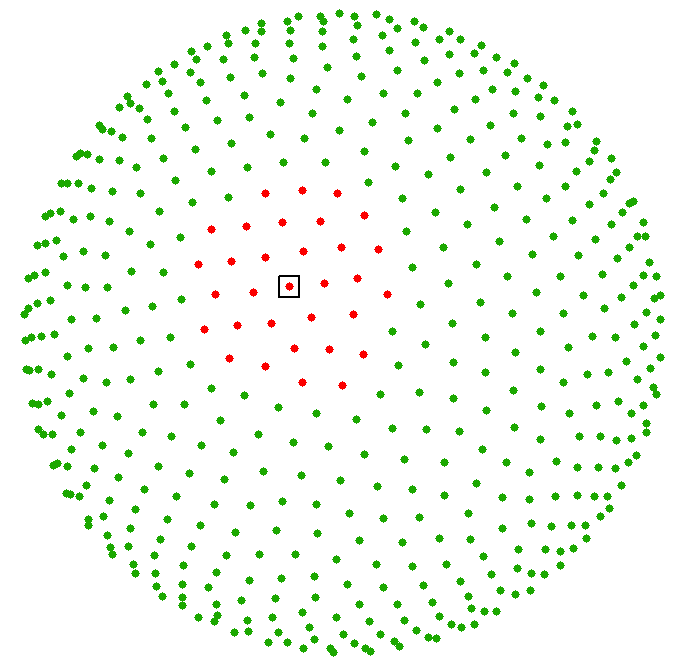
\includegraphics[width=0.8\linewidth]{figures/RBFStencil_n32_a}\label{fig:stencil}
\caption{An example of an RBF-FD stencil of size $n=32$ on a sphere of $N=1024$ nodes to approximate any derivative operator at the point in the square. In nonsparse format, the DM  is $1024\times1024$ with 32 nonzero entries per row.}
\end{figure}


Due to the above attributes and its simplicity of implementation, the RBF-FD is gaining popularity in modeling systems of PDEs in a variety of fields in fluid dynamics (e.g., geosciences, combustion, aerodynamics \cite{Bayona13,CDNT,FoL11,FLBWSC12,SPLM}). For example, the full shallow water equations in a 3D Cartesian coordinate system for a rotating fluid are as follows:
{
\small
\begin{eqnarray}
\dfrac{\partial u}{\partial t} &=& - \left( u\dfrac{\partial u}{\partial x} + v\dfrac{\partial u}{\partial y} + w\dfrac{\partial u}{\partial z} + f(yw - zv) + g\dfrac{\partial h}{\partial x} \right) 
\nonumber \\
\dfrac{\partial v}{\partial t} &=& - \left( u\dfrac{\partial v}{\partial x} + v\dfrac{\partial v}{\partial y} + w\dfrac{\partial v}{\partial z} + f(zu - xw) + g\dfrac{\partial h}{\partial x} \right)
\nonumber\\
\dfrac{\partial w}{\partial t} &=& - \left( u\dfrac{\partial w}{\partial x} + v\dfrac{\partial w}{\partial y} + w\dfrac{\partial w}{\partial z} + f(xv - yu) + g\dfrac{\partial h}{\partial x} \right)
\nonumber\\
\frac{\partial h}{\partial t}& =&-\left(\dfrac{\partial (uh)}{\partial x} + \dfrac{\partial (vh)}{\partial y} + h\dfrac{\partial (wh)}{\partial z}\right) , \label{height} \nonumber
\end{eqnarray}
} where $f$ is the Coriolis force, $\{u,v,w\}$ are the components of the velocity vector in the respective $\{x,y,z\}$ directions, and $h$ is the geopotential height (analogous to pressure). Thus, we have four variables $\{u,v,w,h\}$ and three DMs, $D_x, D_y, D_z$ representing $\dfrac{\partial}{\partial x}, \dfrac{\partial}{\partial y},\dfrac{\partial w}{\partial z}$, respectively. Moreover, in order to stably time step the equations with an explicit time-stepping scheme, most numerical methods (including RBF-FD) require a fourth operator, hyperviscosity, to be added to each equation. Hyperviscosity takes the form of $\triangle^p$ ($\triangle$ denotes the Laplacian operator), where $p\geq3$, which is approximated by the matrix $D_{hyp}$. Therefore, in order to solve this system of PDEs, the application of 4 DM to 4 unknowns, i.e. 16 SpMV is required at every time step. Due to the fact that RBFs are independent of a coordinate system, taking into account only distances to nearest neighbors, the DMs have the following properties:
\begin{itemize}
\item For a given $n$, regardless of the operator approximated, e.g. $\dfrac{\partial}{\partial x}$ or the Laplacian, RBF-FD DMs will have the same number of nonzeros per row.
\item For a given $n$ and $N$, regardless of the operator approximated, the DMs will have the same sparsity pattern. Examples of an RBF-FD DM can be seen in Figures \ref{fig:spy_plots}d and e.
\end{itemize}



Multiple variables transform a SpMV into a SpMM (Sparse Matrix/dense Matrix multiplication), which improves register utilization and decreases cache
misses by vectorizing over the multiple source vectors. Furthermore, due to the properties just mentioned, multiple derivatives of a single function can be calculated rather than computing a single derivative of multiple functions. Using the PDE system above as an example, the block structure of the SpMM for computing all derivatives needed is %can be seen in Equation \ref{fig:struct_comp}, 
%\begin{figure}[h]
\begin{equation}
  %\centering
 %{\small
   \left( \begin{array}{cccc}
    \underline{u}_x     & \underline{v}_x     & \underline{w}_x     & \underline{h}_x \\
    \underline{u}_y     & \underline{v}_y     & \underline{w}_y     & \underline{h}_y \\
    \underline{u}_z     & \underline{v}_z     & \underline{w}_z     & \underline{h}_z \\
    \underline{u}_{hyp} & \underline{v}_{hyp} & \underline{w}_{hyp} & \underline{h}_{hyp}
  \end{array} \right)
  = \left(
  \begin{array}{c}
    D_{x}\\ D_{y}\\ D_{z}\\ D_{hyp}
  \end{array}\right)
  \times \left(\underline{u} \,\, \underline{v} \,\, \underline{w} \,\, \underline{h} \,\,\right) 
  \vspace{-1ex}
  %\caption{Block structure of the computation.}
  \label{fig:struct_comp}
%\end{figure}
\end{equation}
where $\{\underline{u},\underline{v}, \underline{w}, \underline{h}\}$ are the functions values at all nodes of the corresponding variables with the left hand side being the resulting derivative approximations. The increased memory bandwidth due to an increase in the number of derivative matrices is offset by improved cache utilization, leading to an overall performance benefit. In practice however, the number of vectors whose derivatives are required is limited, capping the performance of the matrix/vector multiplication. Similarly, the number of different derivatives in a particular computation is finite. It is for this reason that we seek to combine the benefits of multiple vectors and multiple matrices simultaneously. We limit this initial study to four vectors and four matrices, which is a common number found in fluid dynamic calculations.

\ge{We also note that the DMs are time-independent. They are computed once \ee{at the beginning of the simulation} and used repeatedly to update the solution 
in time \ee{(for each iteration of the simulation)}. Thus, the cost to calculate the derivatives, although high, is amortized by the very long numerical simulations.}

%\end{document}

%
\section{Derivatives of Radial Basis Functions}
\label{sec:rbf}

In this paper, we propose a new idea that is applicable to radial
basis functions (RBFs). Their strength is the ability to randomly
distribute points across complex physical domains, and have an
implementation that is independent of dimensionality. RBFs approximate
a function $f(\rvec)\subset \mathbb{R}^d$ sampled at a set of $N$
distinct point locations, $x_j$, by linearly combining translates of a
single radially symmetric function $\phi(r)$, where $r =
\|\rvec-\rvec_{j}\|$ denotes the Euclidean distance %(e.g., in 2-D
%$\sqrt{(x-x_j)^2+(y-y_j)^2}$) 
between $\rvec$, where the function is evaluated
and and $\rvec_j$,  where the RBF is centered. That is, the
interpolant is $s(\rvec) = \sum_{j=1}^{N} w_j
\phi_i(\|\rvec-\rvec_{j}\|)$. The weights $w_j$ are obtained by
inverting the system
\begin{equation}
\parray{lccr}{
\phi_{11} & \phi_{12} & \cdots & \phi_{1N} \\
\vdots & \ddots & \vdots & \vdots \\
\phi_{n1} & \phi_{n2} & \cdots & \phi_{NN} 
}
\parray{c}{ w_{1} \\ \vdots \\ w_{N} }
=
\parray{c}{ f(\rvec_1) \\ \vdots\\ f(\rvec_N) }. 
\label{eq:rbf}
\end{equation}
where $\phi_{ij} = \phi(\|\rvec_i-\rvec_j\|)$. 

The RBF differentiation matrix, $D_N$, is derived by applying the
desired analytic derivative operator $L$ to the RBF interpolant
$s(\rvec)$ above and evaluating it at the point locations. For very
large problems, this is a computationally expensive since the matrix
in (\ref{eq:rbf}) is full and inversion requires O$(N^3)$
operations. To alleviate the cost of this global approach (i.e., using
every node in the domain to calculate the derivative at a given node
$\rvec_i$), RBF-generated finite differences (RBFFD) have been
derived \cite{TAI1,TAI2,SDY02,WrFo06,FoL11,FLBWSC12}. RBFFD uses only
a local set of the $n_z-1$  (often nearest) points in a neighborhood of 
the point $\rvec_i$ to
approximate the derivative. In other words,
$Lf(\rvec_i)=\sum_{j=1}^{n_z}a_jf(\rvec_j)$. The differentiation
weights, $a_j$, are calculated by enforcing that this linear
combination should be exact for RBFs,
$\{\phi(\|\rvec-\rvec_{j}\|)\}_{j=1}^{n_z}$, centered at each of the
node locations $\{\rvec_j\}_{j=1}^{n_z}$ (classical finite-differences
(FD) would enforce that it be exact for polynomials instead.) Similar
to FD, as the stencil size $n_z$ increases so does the order of the
method.

For a total of $N$ points, there will be $N$ linear systems to solve,
each of size $n_z \times n_z$. Each linear solve produces a row of the
RBFFD differentiation matrix $A_{n_z}$, resulting in a $N \times N$
matrix with $n_zN$ nonzero entries. To evaluate the derivative at all
points in the domain, one multiplies the source vector $x$ by the 
derivative matrix $A$ to obtain the vector $y$ of derivative values, 
$$
  y = A x
$$
The computation of a single derivative has been reduced to a SpMV, 
where each row has $n_z$ nonzeros\footnote{We use non-conventional 
symbology for the differentiation matrix, source and destination vectors, 
anticipating what follows.}. 
In practice, $n_z=32$ in two-dimensional flows and 64 or 100 for
three-dimensional flows. These numbers are on par with what is used in
finite-element codes. Notice that the nonzero elements of the matrix
correspond to a relationship of closeness in the physical domain. 
This relationship is not
necessarily symmetric as shown in Figure~\ref{fig:rbf_stencils}, which
implies a non-symmetric sparsity pattern in the derivative matrix. 

\begin{figure}[tbh]
  \centering
  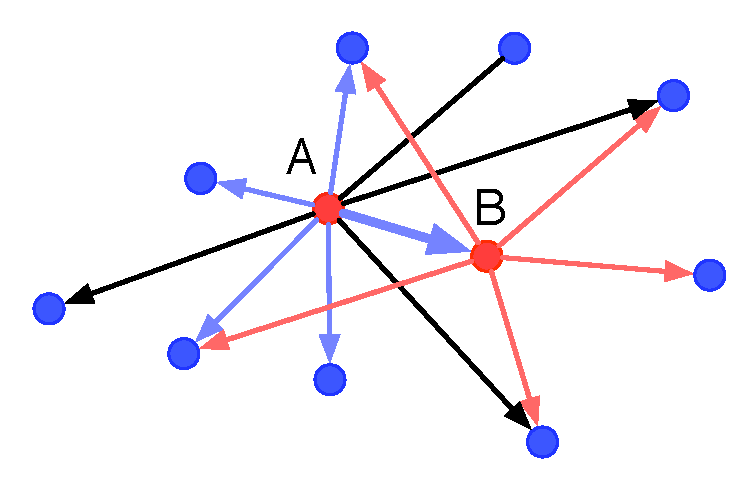
\includegraphics[width=.8\linewidth]{figures/rbf_stencils.pdf}
  \caption{RBFFD Stencils. Each node of the stencil is connected to
    $n_z-1$ stencil nodes in addition to itself. In the figure, node
    $A$ is connected to $B$, but $B$ is {\em not\/} connected to
    $A$. Thus adjacency graph of $A$ is not-symmetric.}
  \label{fig:rbf_stencils}
\end{figure}

Many problems in fluid dynamics and in the geosciences require the
solution to transport equations of the form
\begin{equation}
\pf{Q}{t} = f(Q,\grad{Q},\Laplacian{Q})  \label{eq:Q}
\end{equation}
where $Q$ is a vector of unknowns.
For example, in solving a system of equations, it is
often necessary to compute the derivative of multiple functions along
the same coordinate direction,
typically four for the Euler equations, or five for the Navier-Stokes
equations. Multiple right-hand sides transform a SpMV into a SpMM
(Sparse Matrix/dense Matrix multiplication), which improves register
utilization and decreases cache misses by vectorizing over the
multiple source vectors. Further improvements are possible by
recognizing that different derivative matrices (e.g., gradient and 
Laplacian operators), 
have the same sparsity distribution as long as the derivative stencils
remain unchanged; only the values in the sparse matrix vary. 
Thus, rather than computing a derivative of multiple
functions, one can calculate multiple derivatives of a single
function. The increased memory bandwidth due to an increase in the
number of derivative matrices is offset by better cache utilization,
leading to an overall performance benefit. In practice however, the number of 
vectors whose derivatives are required is limited, capping the 
performance of the matrix/vector multiplication. Similarly, the number
of different derivatives in a particular computation is finite. It is 
for this reason that we seek to combine the benefits of multiple
vectors and multiple matrices simultaneously. We limit this initial 
study to four vectors and four matrices. 

In discrete form, Equation (\ref{eq:Q}) becomes
$$
  y^{i,j} = A^i x^j 
$$ where $j$ ranges over the number of source vectors, $i$ ranges of
  the number of derivative matrices and there are $i*j$ output vectors
  $y$ (graphically shown in Figure~\ref{fig:struct_comp}).

\begin{figure}
  \centering

  \[ \left( \begin{array}{cccc}
    y^{1,1} & y^{1,2} & y^{1,3} & y^{1,4} \\
    y^{2,1} & y^{2,2} & y^{2,3} & y^{2,4} \\
    y^{3,1} & y^{3,2} & y^{3,3} & y^{3,4} \\
    y^{4,1} & y^{4,2} & y^{4,3} & y^{4,4} 
  \end{array} \right)
  = \left(
  \begin{array}{c}
    A^1\\
    A^2\\
    A^3\\
    A^4
  \end{array}\right)
  \times \left(x^1 x^2 x^3 x^4 \right) \] 
  
  \caption{Structure of the computation.}
  \label{fig:struct_comp}
\end{figure}




\section{Introduction and Motivation for RBF-FD}
\label{sec:rbf}

RBFs approximate a function $f(\mathbf{x}) \in \mathbb{R}^d$ sampled at $N$ distinct node locations by linearly combining translates of a single radially symmetric function, e.g. $\phi(r) = e^{-\varepsilon^2r^2}$, where $r=\|\mathbf{x}-\mathbf{x}_{i}\|$ denotes the Euclidean distance between where the function $f(\mathbf{x})$ is evaluated, $\mathbf{x}$, and where the RBF, $\phi$, is centered $\mathbf{x}_{i}$. The parameter $\varepsilon$ controls the shape of the RBF. Note that the argument of an RBF is simply a scalar distance, $r$, independent of any coordinate system or dimension. As a result, nodes can be scattered as desired across complex physical domains with the implementation of the method being independent of dimensionality. Thus, no mesh generation is needed and algorithmic complexity does not increase with dimension.
\NOTE{While reading that paragraph, I was under the impression that the physical domain needs to be a sphere.}

To obtain a RBF derivative approximation at a node location that will result in a sparse differentiation matrix (DM), the RBF-FD method has been developed over the last decade \cite{TAI1,TAI2,SDY02,WrFo06}. RBF-FD is conceptually similar to standard finite differences (FD). 
However, the differentiation weights for approximating a derivative at a given node (forming one row of the RBF-FD derivative matrix (DM)) enforce that the linear combination of function values at the $n << N$ nearest node locations (a stencil) be exact for RBFs centered at each of the $n$ nodes rather than polynomials. The result is a sparse matrix with only $n$ entries in each of its $N$ rows, resulting in a total of $nN$ nonzero entries. An example stencil is shown in 
%Figure~\ref{fig:stencil}.  % Latex is making this figure 2. Do not know why. 
Figure~1.

\begin{figure}[t]
\centering
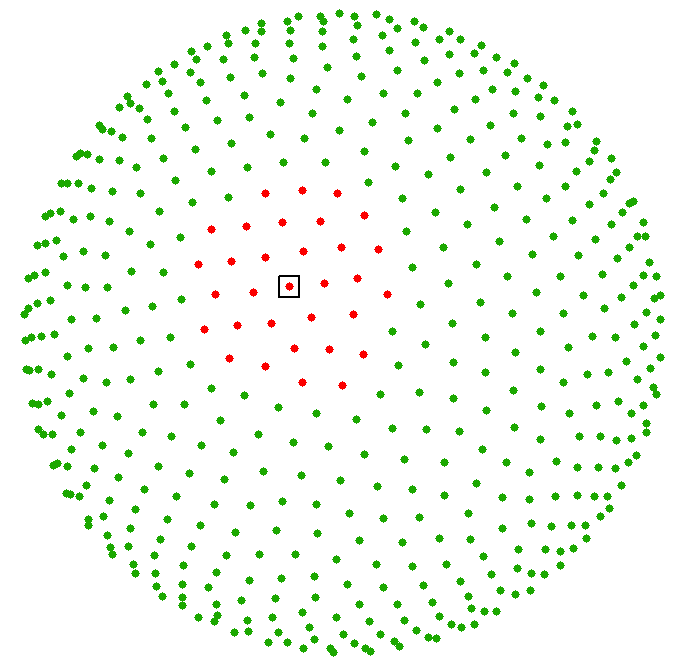
\includegraphics[width=0.65\linewidth]{figures/RBFStencil_n32_a}\label{fig:stencil}
\caption{An example of an RBF-FD stencil of size $n=32$ on a sphere of $N=1024$ nodes to approximate any derivative operator at the point in the square. In nonsparse format, the DM  is $1024\times1024$ with 32 nonzero entries per row.}
\end{figure}

Due to the above attributes and its simplicity of implementation, the RBF-FD is gaining popularity in modeling systems of PDEs in a variety of fields in fluid dynamics (e.g., geosciences, combustion, aerodynamics \cite{Bayona13,CDNT,FoL11,FLBWSC12,SPLM}). For example, the full shallow water equations in a 3D Cartesian coordinate system for a rotating fluid are as follows:
{ \small
\begin{eqnarray}
\dfrac{\partial u}{\partial t} &=& - \left( u\dfrac{\partial u}{\partial x} + v\dfrac{\partial u}{\partial y} + w\dfrac{\partial u}{\partial z} + f(yw - zv) + g\dfrac{\partial h}{\partial x} \right) 
\nonumber \\
\dfrac{\partial v}{\partial t} &=& - \left( u\dfrac{\partial v}{\partial x} + v\dfrac{\partial v}{\partial y} + w\dfrac{\partial v}{\partial z} + f(zu - xw) + g\dfrac{\partial h}{\partial x} \right)
\nonumber\\
\dfrac{\partial w}{\partial t} &=& - \left( u\dfrac{\partial w}{\partial x} + v\dfrac{\partial w}{\partial y} + w\dfrac{\partial w}{\partial z} + f(xv - yu) + g\dfrac{\partial h}{\partial x} \right)
\nonumber\\
\frac{\partial h}{\partial t}& =&-\left(\dfrac{\partial (uh)}{\partial x} + \dfrac{\partial (vh)}{\partial y} + h\dfrac{\partial (wh)}{\partial z}\right) , \label{height} \nonumber
\end{eqnarray}
}
where $f$ is the Coriolis force, $\{u,v,w\}$ are the components of the velocity vector in the respective $\{x,y,z\}$ directions, and $h$ is the geopotential height (analogous to pressure). Thus, we have four variables $\{u,v,w,h\}$ and three DMs, $D_x, D_y, D_z$ representing  $\partial_x$, $\partial_y$, $\partial_z$, 
%\begingroup
%\everymath{\footnotesize}
%\scriptsize
%$\dfrac{\partial}{\partial x}, \dfrac{\partial}{\partial y},\dfrac{\partial}{\partial z}$, 
%\endgroup
respectively. Moreover, in order to stably time step the equations with an explicit time-stepping scheme, most numerical methods (including RBF-FD) require a fourth operator, hyperviscosity, to be added to each equation. Hyperviscosity takes the form of $\triangle^p$ ($\triangle$ denotes the Laplacian operator), where $p\geq3$, which is approximated by the matrix $D_{hyp}$. Therefore, in order to solve this system of PDEs, the application of 4 DM to 4 unknowns, i.e. 16 SpMV is required at every time step. Due to the fact that RBFs are independent of a coordinate system, taking into account only distances to nearest neighbors, the DMs have the following properties:
\begin{itemize}
\item For a given $n$, regardless of the operator approximated, e.g.,
$\partial_x$, 
%$\dfrac{\partial}{\partial x}$ 
or the Laplacian, RBF-FD DMs will have the same number of nonzeros per row.
\item For a given $n$ and $N$, regardless of the operator approximated, the DMs will have the same sparsity pattern. Examples of an RBF-FD DM can be seen in Figures \ref{fig:spy_plots}d-e.
\end{itemize}


Multiple variables transform a SpMV into a SpMM (Sparse Matrix/dense Matrix multiplication), which improves register utilization and decreases cache
misses by vectorizing over the multiple source vectors. Furthermore, due to the properties just mentioned, multiple derivatives of a single function can be calculated rather than computing a single derivative of multiple functions. Using the PDE system above as an example, the block structure of the SpMM for computing all derivatives needed is %can be seen in Equation \ref{fig:struct_comp}, 
%\begin{figure}[h]
\begingroup
\everymath{\footnotesize}
\scriptsize
\begin{equation}
  %\centering
 %{\small
   \left( \begin{array}{cccc}
    \underline{u}_x     & \underline{v}_x     & \underline{w}_x     & \underline{h}_x \\
    \underline{u}_y     & \underline{v}_y     & \underline{w}_y     & \underline{h}_y \\
    \underline{u}_z     & \underline{v}_z     & \underline{w}_z     & \underline{h}_z \\
    \underline{u}_{hyp} & \underline{v}_{hyp} & \underline{w}_{hyp} & \underline{h}_{hyp}
  \end{array} \right)
  = \left(
  \begin{array}{c}
    D_{x}\\ D_{y}\\ D_{z}\\ D_{hyp}
  \end{array}\right)
  \times \left(\underline{u} \,\, \underline{v} \,\, \underline{w} \,\, \underline{h} \,\,\right) 
  \vspace{-1ex}
  %\caption{Block structure of the computation.}
  \label{fig:struct_comp}
%\end{figure}
\end{equation}
\endgroup
where $\{\underline{u},\underline{v}, \underline{w}, \underline{h}\}$ are the functions values at all nodes of the corresponding variables with the left hand side being the resulting derivative approximations. The increased memory bandwidth due to an increase in the number of derivative matrices is offset by improved cache utilization, leading to an overall performance benefit. In practice however, the number of vectors whose derivatives are required is limited, capping the performance of the matrix/vector multiplication. Similarly, the number of different derivatives in a particular computation is finite. It is for this reason that we seek to combine the benefits of multiple vectors and multiple matrices simultaneously. We limit this initial study to four vectors and four matrices, which is a common number found in fluid dynamic calculations. Equation~\ref{fig:struct_comp} is of the form $Y=AX$, where $Y$ encodes the $x,y,z$ discrete derivatives (and hyperviscosity operator) of $u,v,w,h$, $X$ encodes the variables $(u,v,w,h)$ and $A$ represents the 16 discrete differentiation operators. 

We also note that the DMs are time-independent. They are computed once \ee{at the beginning of the simulation} and used repeatedly to update the solution 
in time (for each iteration of the simulation). Thus, the cost to calculate the derivatives, although high \ger{(on the order of 1000 SpMVs)}, 
is amortized by the very long numerical simulations. \ger{The startup cost is eliminated when performing parameter studies on a given node distribution. Furthermore, the computation of the derivative matrices are done serially, but are trivially parallelizable.}


%--------------------------------------------
\section{Modeling the\\ Potential Improvements}
\label{sec:model}

We saw in the previous section that one can express the RBF problem as
a multiplication of four matrices by four vectors. We present here an
estimation of the variation on the flop intensity of the computation
and its impact on the expected performance of the
application. Relevant notation are given in Figure~\ref{tab:not}.

\begin{figure}[tbh]
  \begin{center}
    \scalebox{.8}{
      \begin{tabular}{|c|l|}
        %\hline
        %& & \\
        \hline
        $b_i$ & number of bytes per index \\
        $b_x$ & number of bytes per value \\
        $n_z$ & number of nonzeros per row of $A$ \\
        $n_r$ & number of column/rows of $A$ \\
        $n_c$ & total number of nonzeros\\
        $n_v$ & number of {\tt x} vectors \\
        $n_m$ & number of matrices \\
        $s_M$ & size of the $n_m$ matrices in bytes\\
        $s_x$ & size of the $n_v$ {\tt x} vectors in bytes\\
        $s_y$ & size of the $n_v n_m$ {\tt y} vectors in bytes\\
        \hline
        $cl$    & size of a cache line in bytes\\
        $b_{wT}$ & number of bytes written to memory  \\
        $b_{rT}$ & minimum number of bytes read from memory  \\
        $b_T$   & minimum number of bytes transferred \\
        $B_{rT}$ & maximum number of bytes read from memory \\
        $B_T$   & maximum number of bytes transferred \\
        $O$     & number of floating point operations \\
        $I_b$   & maximum computational intensity\\
        $I_w$   & minimum computational intensity\\        
        \hline
      \end{tabular}
    }
  \end{center}
  \caption{Notation relative to the application problem (upper section) and to the benchmarks (lower section.)}
  \label{tab:not}
\end{figure}

Each vector in the problem is of dimension $n_r$ and each entry
takes $b_x$ bytes. There are $n_v$ {\tt x} vectors and $n_v n_m$ {\tt
  y} vectors, which lead to the size of the {\tt x} and {\tt y} vectors:
$$s_x = n_v b_x n_r\mbox{, ~}s_y = n_v n_m b_x n_r$$

The matrix is composed of $n_r$ rows and columns with $n_z$ nonzeros
per row leading to a total of $$n_c = n_r n_z$$ nonzero entries in
the matrix. Each of these nonzero entries has one index of size $b_i$
and $n_m$ values of size $b_x$. The matrices have a total size
of $$s_M = n_c (b_i + b_x n_m) = n_r n_z (b_i + b_x n_m)$$

\begin{figure*}[tbh]
  \centering
  \subfigure[Best case.]{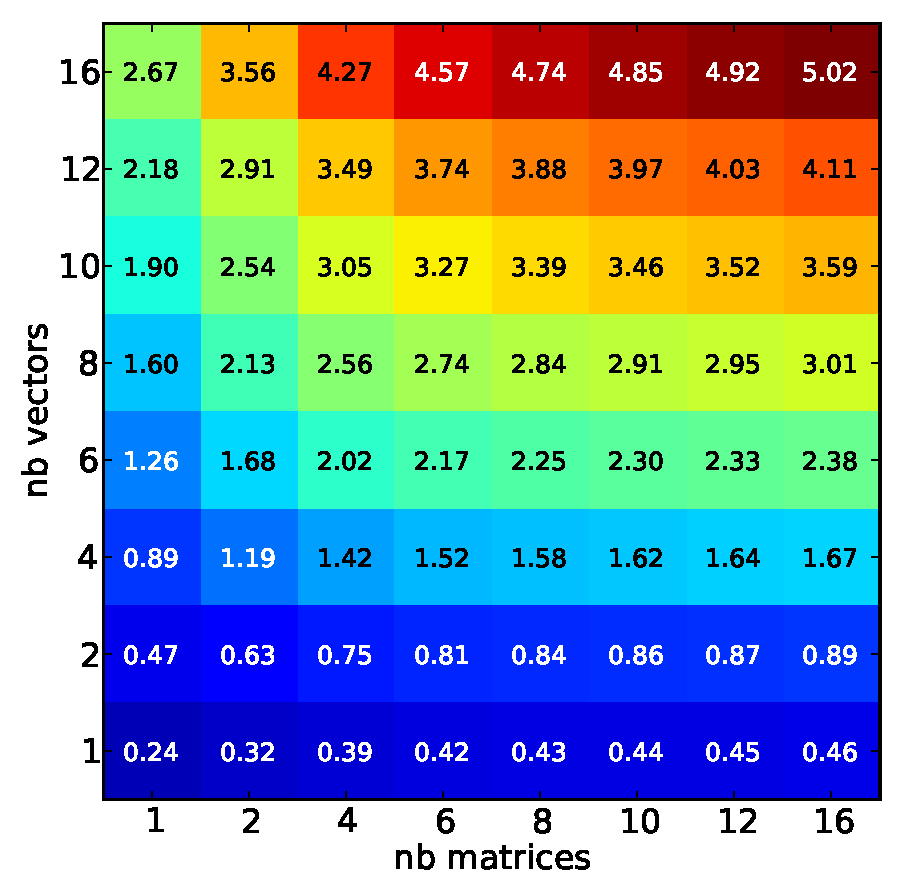
\includegraphics[width=.33\linewidth]{figures/flops_to_bytes_best-crop.pdf}\label{fig:ratio_best}}%
  \subfigure[Worst case.]{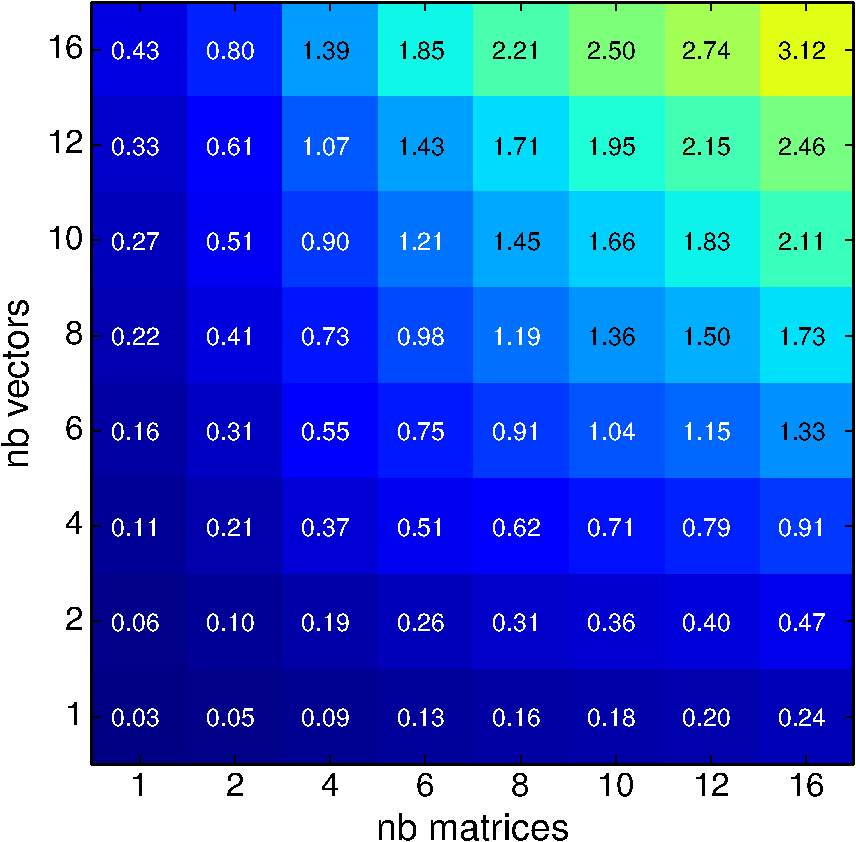
\includegraphics[width=.33\linewidth]{figures/flops_to_bytes_worst-crop.pdf}\label{fig:ratio_worst}}%
  \subfigure[Worst case (No cacheline effects)]{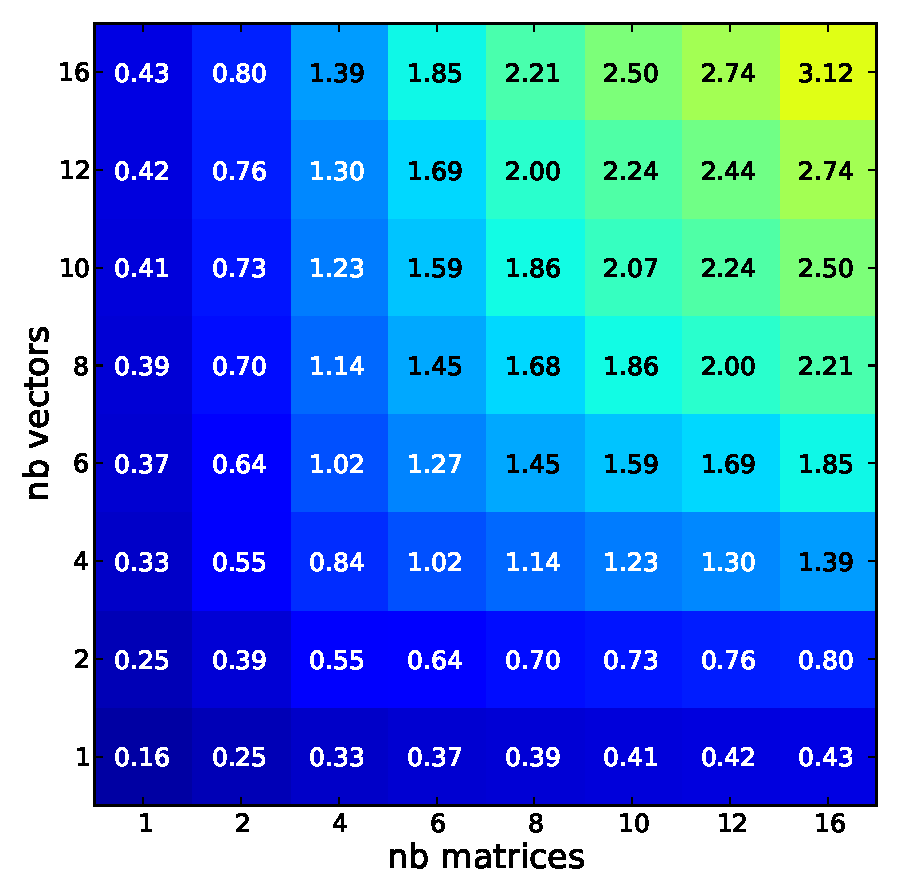
\includegraphics[width=.33\linewidth]{figures/flops_to_bytes_no_cache-crop.pdf}\label{fig:ratio_worst_nocache}}
  
  \caption{Ratio of flops to bytes in single precision:  
    \ref{fig:ratio_best} best case; \ref{fig:ratio_worst} worst case when $cl=64$ 
    ; and \ref{fig:ratio_worst_nocache} worst case neglecting that the
    memory transfers are with a granularity of one cache line (equivalent to $cl = 1$)}
  \label{fig:ratio_bytes_flops}
\end{figure*}


If we assume an algorithm where the rows are processed one after
the other, the amount of memory written is precisely the
size of the {\tt y} vector. (This assumption removes the possibility of
blocking or cache partitioning techniques.) $$b_{wT} = s_y = n_v n_m b_x n_r$$

The amount of data read from memory depends highly on both the
algorithm's execution path, and on how the matrix is structured. But
in the best case both the matrix $A$ and the source vector {\tt x} are
read once from the main memory. (We assume that all the elements of
$\tt x$ are involved in the SpMV.)  Thus, $$b_{rT} = s_M + s_x = n_r
n_z (b_i + b_x n_m) + n_v b_x n_r$$
 $$b_T = b_{rT} + b_{wT} =  n_r n_z (b_i + b_x n_m) + n_v b_x n_r (1 + n_m)$$

Notice that there is no reason for a piece of the matrix to be read
multiple times. But assuming that each element of the {\tt x} vector
is read a single time is a strong assumption. If using a single core,
it assumes that either the cache of the architecture can store the full
{\tt x} vector or that the matrix is sufficiently well structured 
to cause no cache trashing. If using multiple cores, this assumes that
no element of the {\tt x} vectors will be used by multiple
cores. \cite{Saule13-ARXIV} showed that there is very little cache trashing
in practice; however having elements of the vectors used by
multiple cores can have a significant impact on the performance
(growing with $n_v$).

On the other hand, in the worst case, every time the {\tt x} vector is
accessed, the value needs to be transferred from memory again. So in
total, there are as many transfers as the number of nonzeros in the
matrix. Note however that most architectures cannot read memory a
single byte at a time. Instead, a minimum number of bytes, equal to
the size of a cacheline $cl$, are transferred at once.  When there are
multiple vectors, each nonzero element uses $n_v$ consecutive
entries. In the worst case, the number of bytes read and transferred is
$$B_{rT} = s_M + n_c cl \ceil{\frac{n_vb_x}{cl}} $$ 
$$B_T = n_v n_m b_x n_r + n_r n_z \left ( b_i + b_x n_m +  cl \ceil{\frac{n_vb_x}{cl}} \right)$$

In SpMV, each nonzero of the matrix requires two floating point
operations: one for performing the multiplication and one for
accumulating the result row-wise. Here we are dealing with $n_v n_m$
simultaneous SpMVs and the number of floating point operations is
$$O = 2 n_v n_m n_c = 2 n_v n_m n_z n_r$$

The computation intensity is the amount of floating point operations performed per
byte transferred. In the worst case and in the best case, we have
$$I_b = \frac{O}{b_T} = \frac{2 n_v n_m}{ (b_i + b_x n_m) + n_v n_m b_x n_z^{-1} + n_v b_x n_z^{-1} }$$
%$$I_w = \frac{O}{B_T} = \frac{2 n_v n_m}{n_v n_m b_x n_z^{-1} + \left ( b_i + b_x n_m +  cl \ceil{\frac{n_vb_x}{cl}} \right)}$$
$$I_w = \frac{O}{B_T} = \frac{2 n_v n_m}{(b_i+b_x n_m) + n_v n_m b_x n_z^{-1} + cl \ceil{\frac{n_vb_x}{cl}} }$$


Figure~\ref{fig:ratio_bytes_flops} presents the flop to byte ratios
for single precision computation in the best and the worst case on a
classical cache-based architecture ($cl = 64$) and assuming $cl=1$. We
can easily see the potential improvement in the computational
intensity when the number of matrices or vectors increases. There is a
significant difference between the best and the worst case: there is a
eightfold difference in the one matrix -- one vector ($n_m=n_v=1$) case but that gap closes
with the increase in the number of vectors and matrices to a fourfold
difference in the four matrices and four vectors ($n_m=n_v=4$) case and 1.6 fold in the 
$n_m=n_v=16$ case. 
The ratios computed with $cl = 1$ are mostly
similar to the one with $cl=64$ when the number of vectors is
large. But the differences are important when the number of vectors is
low: this highlights that accessing the memory with a granularity of one cache
line is a main problem faced when performing a standard SpMV computation.

Figure~\ref{fig:perf_predict} shows how these ratios translate
into actual performance. This figure provides projected best and worst
Gflop/s achievable assuming the computation is memory-bound and the
architecture reaches 150~GB/s. Notice that \cite{Saule13-ARXIV}
showed a higher peak bandwidth, but we will show in
Section~\ref{sec:expe} why 150~GB/s is a better estimate of what one
might achieve in these kernels. In single precision, the worse that
one could achieve by using four vectors and four matrices is much higher
than the best achievable using a classical SpMV computation. The best
performance reachable is 210~Gflop/s: almost six times higher than the
peak of the classical SpMV case. 


\begin{figure}[t]
  \centering 
  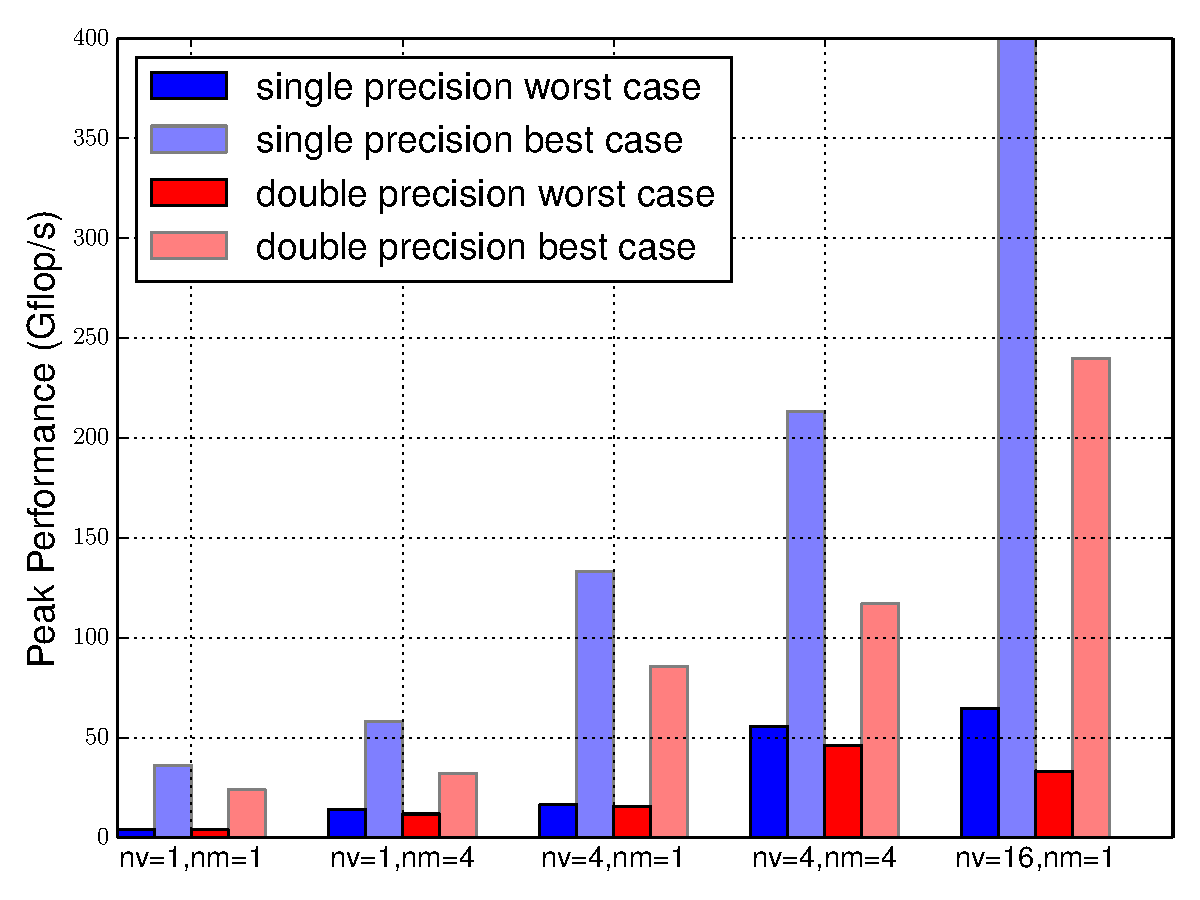
\includegraphics[width=.9\linewidth]{figures/gflops_peak.pdf}\label{fig:gflops-peak-perf}
  \caption{Estimation of the maximum achievable performance using a
    device with a bandwidth from memory to computational units of 150~GB/s when
    varying the number of vectors and matrices.}
  \label{fig:perf_predict}
\end{figure}

\section{Efficient Implementation on the Intel Xeon Phi processor}
\label{sec:impl}

\subsection{Intel Xeon Phi}

In this work, we use an Intel Xeon Phi 5110P coprocessor. This card
has 8 memory controllers that can each execute 5 billion
transactions per second. Each has two 32-bit channels, achieving a total
bandwidth of 320~GB/s aggregated across all the memory
controllers. There are 60 cores clocked at 1.05~GHz. Their memory
interfaces are 32-bit wide with two channels and the total bandwidth
is 8.4~GB/s per core. Thus, the cores should be able to consume 504~GB/s
at most. However, the bandwidth between the cores and the memory
controllers is limited by the ring network that connects the cores and
the memory controller. Its precise bandwidth is
believed to be between 200~GB/s and 250~GB/s.

Each core in the architecture has a 32~kB L1 data cache, a 32~kB L1
instruction cache, and a 512~kB L2 cache. The architecture of a core is
based on the traditional Pentium architecture, which has been extended to
64-bit with hyperthreading. A core can hold four hardware contexts at any given time (240 threads in total). At each
clock cycle, instructions from a single thread are executed. Due to
some hardware constraints, two hardware contexts must be used to reach
the peak instruction throughput in that architecture. Similar to the
Pentium architecture, a core has two different concurrent instruction
pipelines that allow the execution of two instructions per
cycle. However, only one vector or floating point instruction can be
executed per cycle.

Most of the performance of the architecture comes from the vector
processing unit. Each core has 32 512-bit SIMD registers that can be
used for double or single precision, that is, either as a vector of eight
64-bit values or as a vector of 16 32-bit values, respectively. 
\ger{The vector processing unit can perform arithmetic (addition and multiplication) 
instructions making it possible to reach 16 single precision 
(or 8 double precision) operations per cycle. 
The unit also supports Fused Multiply-Add (FMA)
operations, which are typically counted as two operations 
when benchmarking. Therefore, the peak performance of the 5110P
card is one Tflop/s in double precision and two Tflop/s in single
precision. If FMA cannot be used, only half of these rates can be
achieved.}

%addition or %division, and mathematical operations, such as {\tt sin} or
%{\tt sqrt}, making it possible to reach 16 single precision (or 8 double precision)
%operations per cycle.  


\subsection{Bringing the data into the vector register}

\begin{figure*}
  \centering
\scalebox{.8}{
\subfigure[Source code]{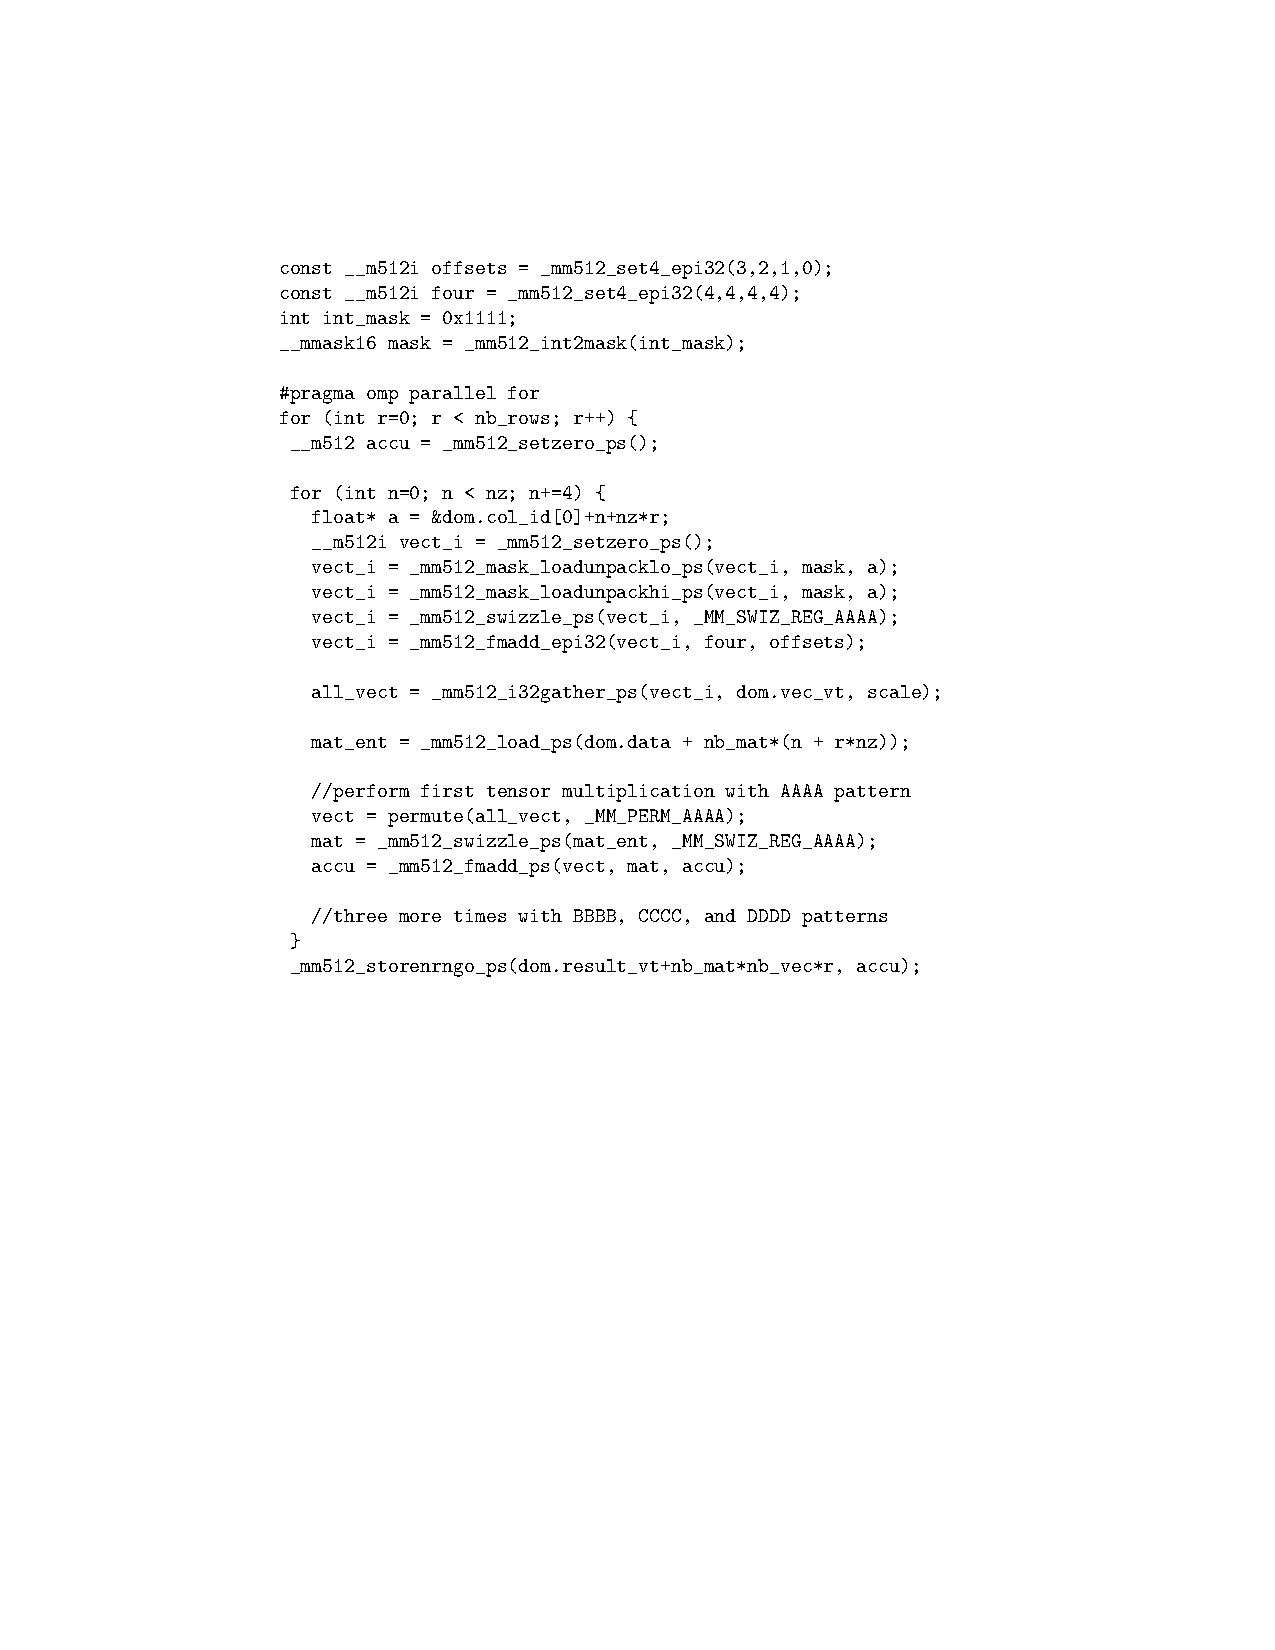
\includegraphics[clip=true,trim=4.5cm 11cm 4cm 4.2cm,width=.6\linewidth]{figures/code.pdf}}%
\subfigure[Content of the vector registers.]{\hspace{0.07\linewidth}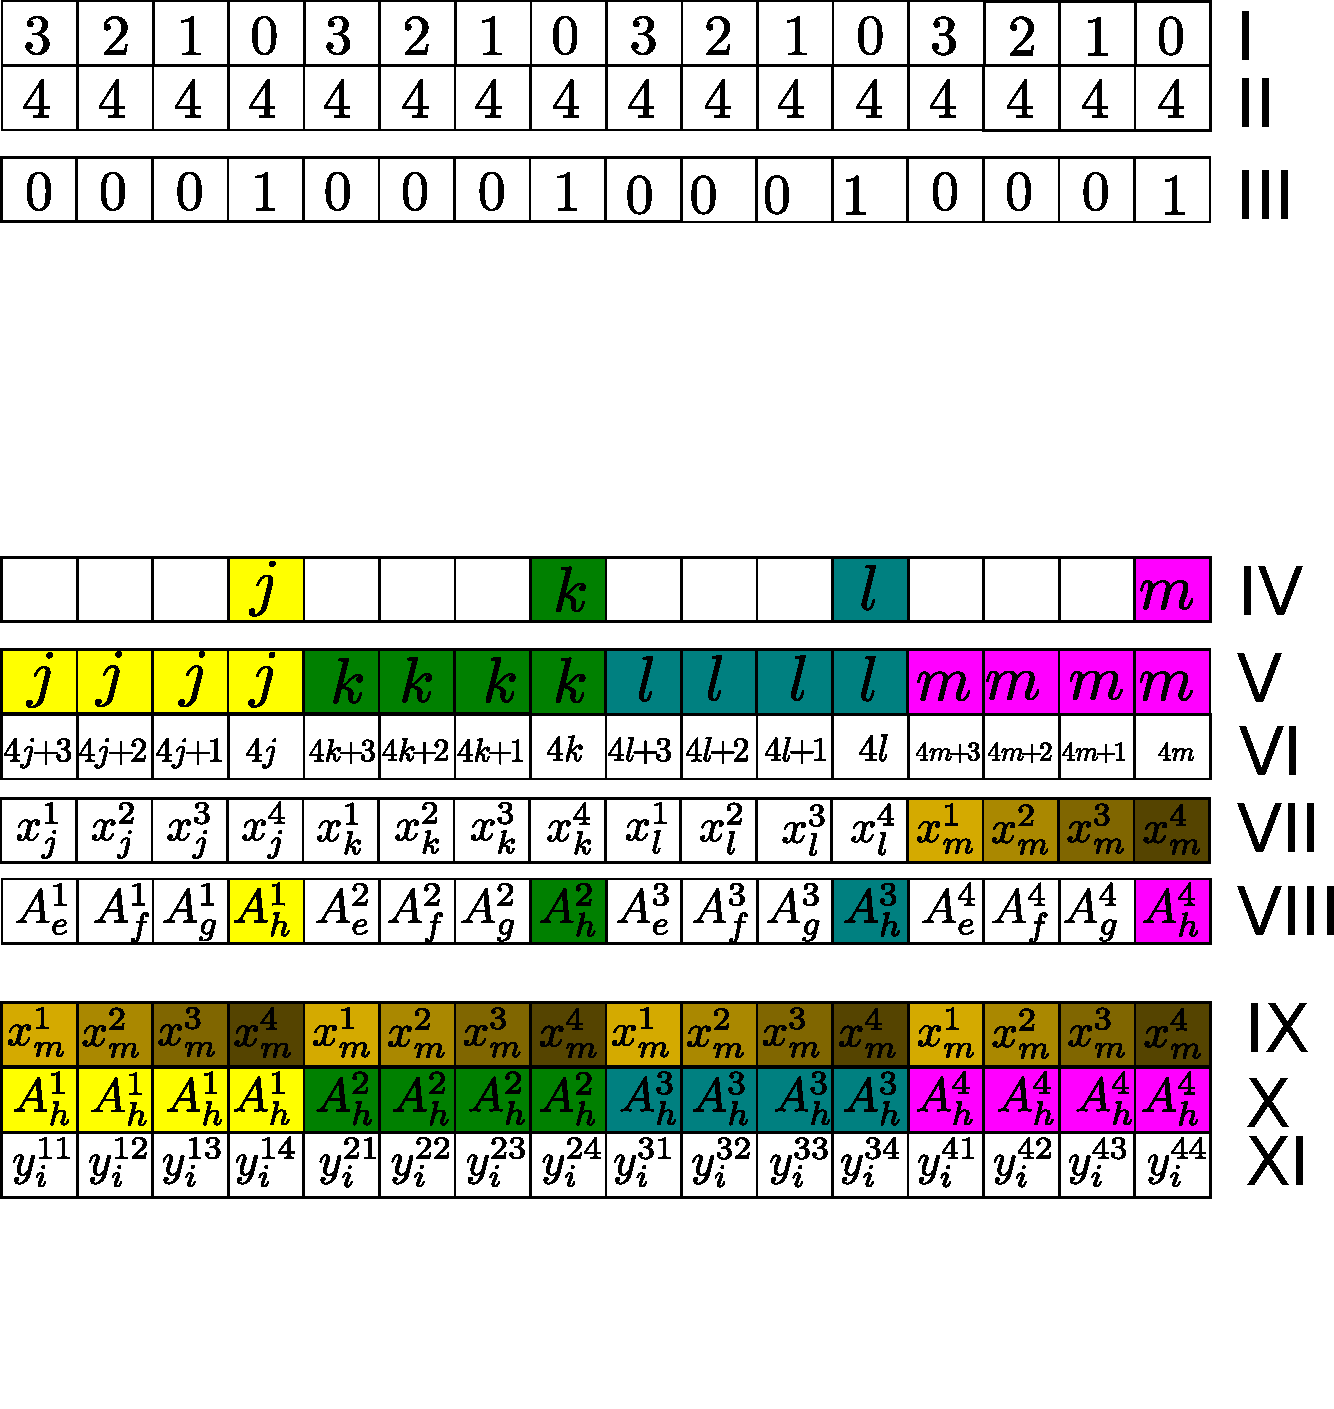
\includegraphics[width=.55\linewidth]{figures/code-annote.pdf}}
%%\subfigure[Content of the vector registers \ge{in the source code}.]{\hspace{-0.07\linewidth}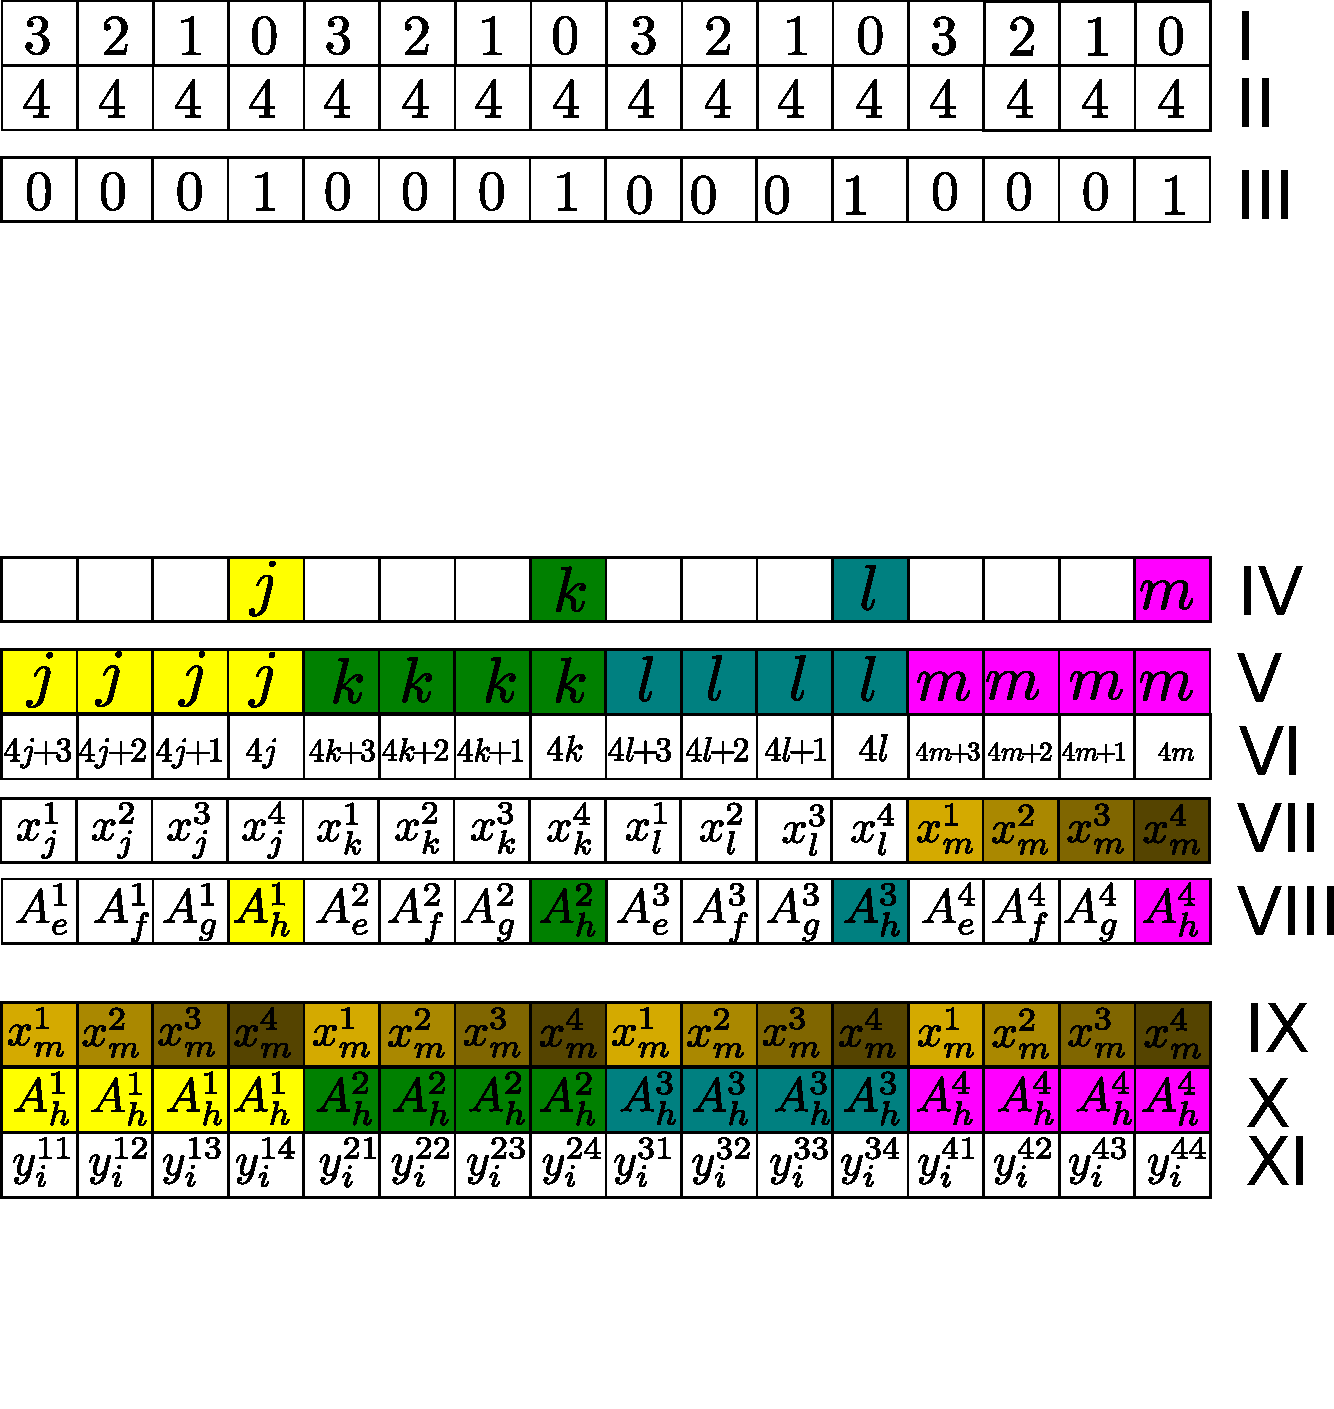
\includegraphics[width=.55\linewidth]{figures/code-annote.pdf}}
}

\caption{Code snippet of the multiplication of 4 vectors with 4
  matrices. When a line changes the content of a vector register its
  new content is shown on the right. The effects of swizzling and
  permutations are highlighted using a color code.}
\label{code:mat_mul}
\end{figure*}



As explained in Section~\ref{sec:model}, we expect to achieve a performance of
about 210~Gflop/s in single precision in the best case. We will focus
on the single precision case with four vectors and four matrices. 
Similar techniques apply for other combinations. This target
performance represents 10\% of the peak performance of the
architecture, which cannot be reached without an efficient vectorization. 
Indeed, to reach such a performance, a Fused Multiply-Add
instruction on fully loaded registers must be executed at most every
10 cycles.

In term of memory layout, we adopt a format similar to the ELLPACK
format to store the matrix since the number of nonzeros per row is
constant throughout the matrix. The matrix is given in two arrays. The
first array is {\tt col\_id} that describes the
sparsity structure of the matrix. Each row of {\tt col\_id} consists
of $n_z$ entries that label the column index of each nonzero in
$A$. %***
The other array is  {\tt data} that gives the values of
the nonzeros in the four matrices. The values of the matrices are
interleaved by groups of four so that the value $A^l_{col\_id[k]}$ of
the $k$th nonzero of the $l$th matrix is at index $\floor{\frac{k-1}{4}}*4*n_m + (l-1)*4+(k-1)\%4$.
(In other words, the first four entries are from $A^{1}$ and the 
next four are from $A^2$.) The vectors {\tt x} are
interleaved so that {\tt x}$^l_i$ and {\tt x}$^{l+1}_i$ are
consecutive in memory. The vector {\tt y} is similarly 
grouped in sets of 16, which correspond to four derivatives applied to
four functions, at a single point. %\ger{All matrices are stored as one-dimensional vectors and pointers to individual rows and elements are explicitely computed.}
\looseness=-1


We discuss how the implementation of the v4m4 kernel works using
vector instructions. The code is given for reference in
Figure~\ref{code:mat_mul} along with a graphical depiction of the content of the registers. (We will show in Section~\ref{sec:expe}
that an implementation that relies on compiler vectorization does not lead
to desirable performance, which confirms the results
of~\cite{Saule13-ARXIV}.) The registers in the MIC architecture are
512 bits wide and can store 16 floats or integers. (In comparison to
OpenCL or CUDA, one can think of these registers as a warp.) The end
goal is to load and format the nonzero values $A_h^1,A_h^2,A_h^3,A_h^4$
and the vector entries $x_m^1,x_m^2,x_m^3,x_m^4$ into two vector registers and 
apply Fused Multiply-Add on them, which is depicted in the {\tt accu} line of 
Figure~\ref{code:mat_mul}. Bringing the data into the vector
register as shown in the figure is the difficult component of our 
proposed algorithm, which we proceed to explain further. 
A thread will perform the multiplications one row at a time,
and parallelism is achieved by giving blocks of rows to each thread
using an OpenMP construct.


\ee{The core of the technique is to load the maximum amount of data
  into large the registers and format the data for processing within these
  registers, minimizing the amount of interaction with memory. 
  The Intel MIC is more for these operations than classical
  CPUs because it features larger vector registers and more elaborate
  vector reorganization instructions, such as swizzling,
  permutations and broadcasts. (The AVX instruction sets on classical
  CPUs are more primitive in that aspect.)} A vector of 512 bits is
composed of four lanes (sometimes called channels) of 128 bits, which
are made of four segments of 32 bits. A swizzling operation allows the
reorder of the elements within each lane (see how {\tt mat} is
extracted from {\tt mat\_ent} in Figure~\ref{code:mat_mul} line VIII to X). On the
other hand, a permutation reorders entire lanes, without changing
their contents (see for instance how {\tt vect} is generated from {\tt
  all\_vect} in Figure~\ref{code:mat_mul} line VII to IX).  Both permutation and
swizzling support common reordering and broadcast. In the code, the
``permute'' function needs to use the {\tt
  \_mm512\_permute4f128\_epi32} instruction which is only defined on
integers and therefore in place typecasts are necessary to convert a
vector to and from integer type.  (Note that we prefer swizzling to
permutation if possible because we believe it is cheaper. Many
instructions have swizzling capability, while permutation is its own
instruction.)

Every operation that loads data from memory into a register
transfers 512 bits, or 16 floats at a time. A single nonzero
in the matrix will cause 16 operations to be performed, but it only
uses four floats from the matrix and four floats from the {\tt x} vector. So
we would like to execute a single instruction to load the data for four 
nonzeros in the matrix, and another instruction to load the data for
four nonzeros from the vectors.  
(The number of nonzeros on a row in our application is
always a multiple of four; if it weren't, we would add some explicit
zeros in the data structure for padding.)

The values from the nonzero elements in the matrix are the simplest to
load. One can load the 16 floating point values for four nonzeros of
the matrix at once. The four floats coming from each matrix are
naturally grouped within each lane of the SIMD register. One can use a
swizzle operation to broadcast the four elements of a single matrix to
fill the whole register. (The broadcast of $A_h^1,A_h^2,A_h^3,A_h^4$ is
shown in Figure~\ref{code:mat_mul}.)

Loading the entries from the {\tt x} vector is  more
involved. First, the column pointers of four different nonzeros are
loaded into a vector register and the values are distributed one per
lane of the vector register using an {\tt unpack}
operation in line IV\footnote{Notice that there are two calls to {\tt unpack} for the
LSB and MSB. Both are mandatory even if one is known to be
nilpotent according the documentation of the hardware.} (The column
pointers are named $j,k,l,m$ in Figure~\ref{code:mat_mul}.) They
are replicated so that each value fills a single vector lane 
using a swizzle operation (in line V). Then each value is multiplied by four
(because $n_v=4$) 
and the offset vector $(3,2,1,0)$ is added to each lane to obtain the
correct index of the elements of the {\tt x} vector within each lane
using a Fused Multiply-Add operation in line VI. A {\tt gather} operation is then
performed in line VII to bring the 16 entries of the {\tt x} vector into the SIMD
register. At this point we have a register where each lane is the
four vector entries for a nonzero element. Using a broadcast
permutation, one can replicate an entry of the four vectors across
each lane. (The broadcast of $x_m^1,x_m^2,x_m^3,x_m^4$ is shown in
Figure~\ref{code:mat_mul} in line IX.)

Now that $A_h^1,A_h^2,A_h^3,A_h^4$ and $x_m^1,x_m^2,x_m^3,x_m^4$ are
properly laid out in the vectors, a partial value for $y_i$ can be
computed in line XI. Once all the nonzeros of the row have been processed, the
exact $y_i$ value can be sent to memory using a the "No Read No Global
Order" hint to optimize write traffic on the memory bus.

\ee{The modelization of Section~\ref{sec:model} establishes that the 
  memory
  transfer caps the computation at 210~GFlop/s, which is 10\% of the
  peak single precision of the architecture. To reach this value, the
  cores need to execute one "useful" Fused Multiply-Add operation
  every ten cycles. The inner loop of the kernel spends 7 vector
  instructions to layout the data and then 3 per tensor product for a
  total of 12 vector instructions. Most of these instruction have a
  one cycle throughput cost except the gather operations which might
  need to perform up to 16 memory accesses. There are also some scalar
  operations but there are few of them and are executed on a different
  pipeline than the vector operations. Overall, the inner loop can
  emit the 4 Fused Multiply-Add in less than 40 cycles.}

\section{Experimental Validation}
\label{sec:expe}

\begin{figure}[t]
  \centering
  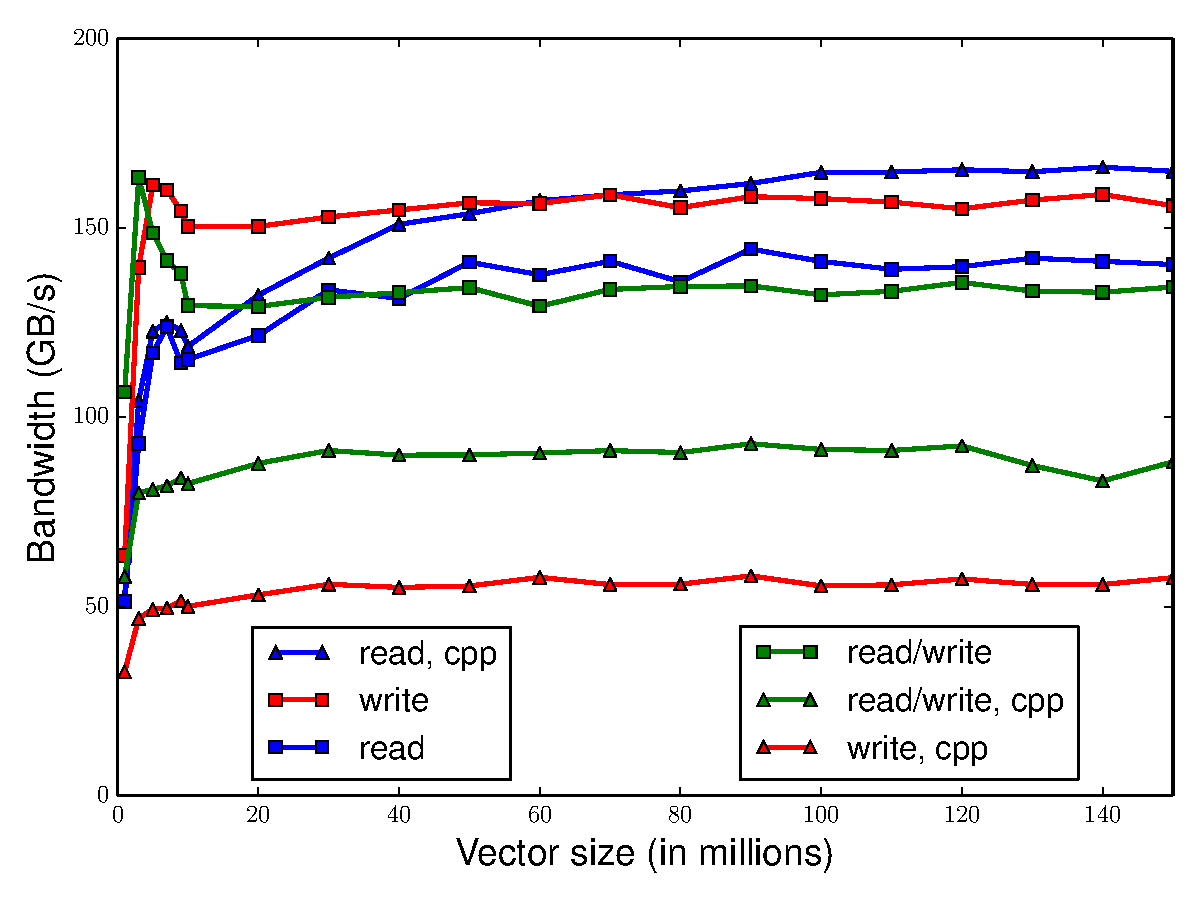
\includegraphics[width=.9\linewidth]{figures/bandwidth_read_write.pdf}
  
  \caption{Bandwidth performance under idealized conditions.  Entries
    with "cpp" (triangles) denote cases where vectorization is
    compiler generated.}
  \label{fig:bandwidth}
  \label{fig:band_rw_MIC}
\end{figure}

In this section, we describe a series of numerical experiments to
confirm the performance predictions of Section~\ref{sec:model}. To
better understand our results, we first perform some bandwidth
measurements, followed by the actual SpMV computations. All the codes
are compiled with the Intel C Compiler version 13 and
\mbox{-O3} optimization. The codes use the IMCI instructions exposed by
the compiler through intrinsics.

\subsection{Bandwidth}


\begin{figure}[t]
  \centering
  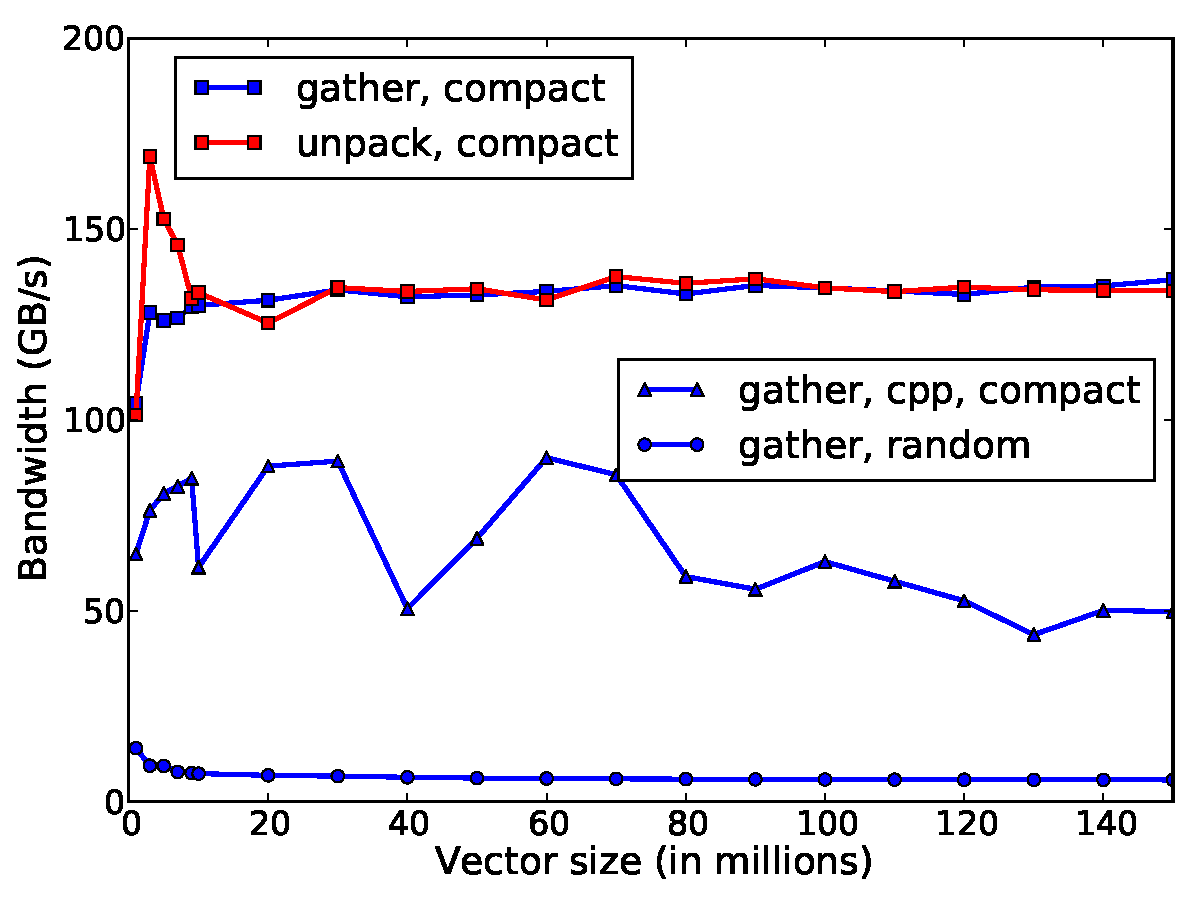
\includegraphics[width=.9\linewidth]{figures/bandwidth_gather_unpack.pdf}
  \caption{Performance of {\tt gather} and {\tt unpack} operations.}
  \label{fig:band_gather} 
\end{figure}


Figure~\ref{fig:bandwidth} shows a benchmark that computes the
bandwidth achieved when reading and/or writing large arrays on 
the MIC card. The read benchmark performs a
simple sum of the array. The write benchmark sets all the elemnts of
the array to zero, while the read/write benchmarks copies the array into
another one. We also investigate the difference between a straight C++
implementation (compiled with \mbox{-O3} with proper tagging to inform the
compiler of memory alignments) and an implementation with
explicit use of the vector registers.

The {\tt read\_cpp} implementation reaches a performance of 168~GB/s
 which is better than the {\tt read}
implementation which only achieves 145~GB/s. This
is explained by the compiler adding loop unrolling and software
prefetching in the assembly code in the {\tt read\_cpp} case, which is
not added in the {\tt read} case. On the other hand, the {\tt write}
case reaches a performance of 158~GB/s while the
{\tt write\_cpp} implementation never exceeds 58~GB/s. 
This difference is the result of {\tt \_mm512\_store\_nrngo\_ps}, 
an instruction, which bypasses the \ge{"Read For Ownership"} protocol 
and allows the writes
to be performed in any order. The compiler can not use this
instruction on its own because this would break the memory convention
useful for some parallel algorithms. The {\tt read/write} benchmark
performs at 140~GB/s while the {\tt read/write\_cpp} benchmark performs
at about 90~GB/s.

Note that SpMV kernels are not likely to use only simple read and simple
writes. We also benchmark the performance we
can achieve using {\tt gather} and {\tt unpack} operations and we
present the results in Figure~\ref{fig:band_gather}. The {\tt unpack}
instruction can reach a performance of 140~GB/s. (There is no easy way
to implement the equivalent of the {\tt unpack} operation without
using explicit registers.) The performance of the {\tt gather}
operations depends in which order the array is read. If the indices
are ordered ({\tt compact}) then a performance of 140~GB/s is
reached. If the indices are completely randomized, the performance
drops below 5~GB/s. We can see that implementing the
indirection mechanism without vector instructions lowers the
performance significantly. (In the {\tt compact} case, it never
surpasses 100~GB/s and is close to 50~GB/s most of the time.)

\def\ww{.19\textwidth}
\begin{figure*}[b]
% Figure 8
  \begin{center}
    \subfigure[Supercompact.]{%
      \label{fig:supercompact}
      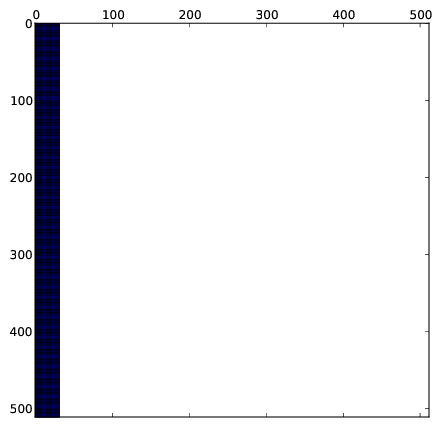
\includegraphics[width=\ww]{figures/supercompact_matrix-crop.png}}%
    \subfigure[Compact.]{%
      \label{fig:compact}
      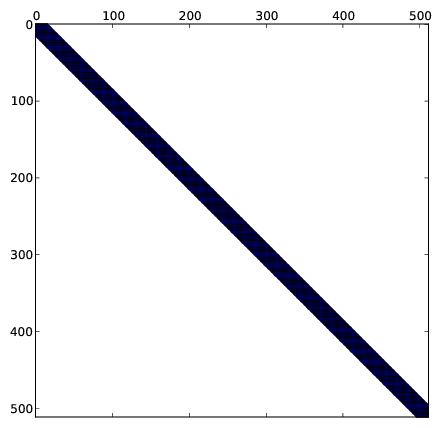
\includegraphics[width=\ww]{figures/compact_matrix-crop.png}}%
    \subfigure[Random.]{%
      \label{fig:random}
      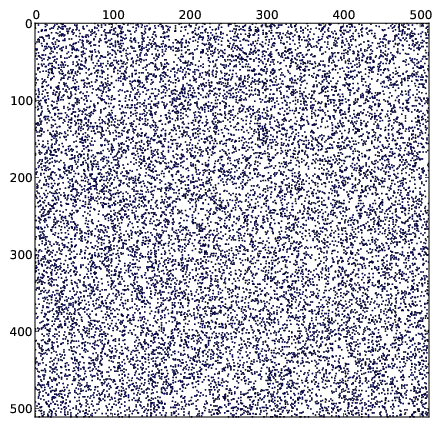
\includegraphics[width=\ww]{figures/random_matrix-crop.png}}%
    %% \subfigure[2D, no RCM.]{%
    %%   \label{fig:rbf2dnorcm}
    %%   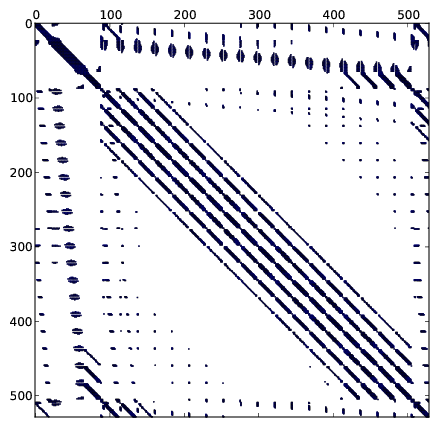
\includegraphics[width=\ww]{figures/kd-tree-2d-norcm-crop.png}}%
    %% \subfigure[2D, RCM.]{%
    %%   \label{fig:rbf2drcm}
    %%   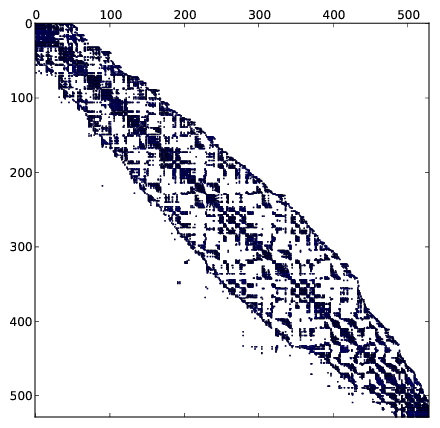
\includegraphics[width=\ww]{figures/kd-tree-2d-rcm-crop.png}} 
    \subfigure[3D, \ge{no RCM}.]{%
      \label{fig:rbf3dnorcm} 
      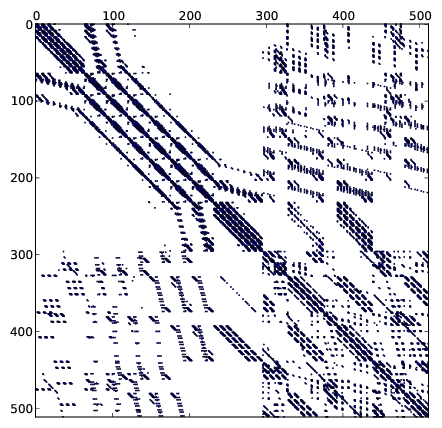
\includegraphics[width=\ww]{figures/kd-tree-3d-norcm-crop.png}}%
    \subfigure[3D, \ge{RCM}.]{%
      \label{fig:rbf3drcm}
      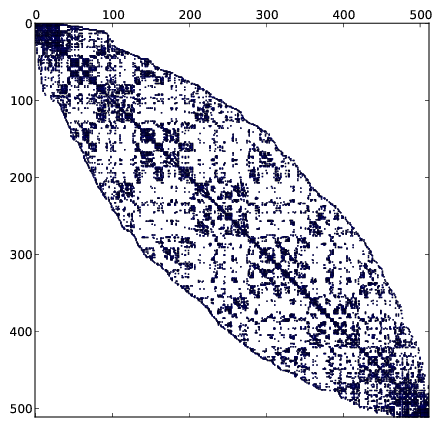
\includegraphics[width=\ww]{figures/kd-tree-3d-rcm-crop.png}}%
  \end{center}
  
  \caption{Different sparsity distributions. In all cases, there are
    512 rows and 32 nonzeros per row. The last two matrices
    corresponds to a derivative stencil in 3D RBFFD
    calculations (with and without RCM ordering).}
  \label{fig:spy_plots}
\end{figure*}

\begin{figure*}
% Figure 9
  \centering
% was width=.48
  \subfigure[Supercompact and Random.]{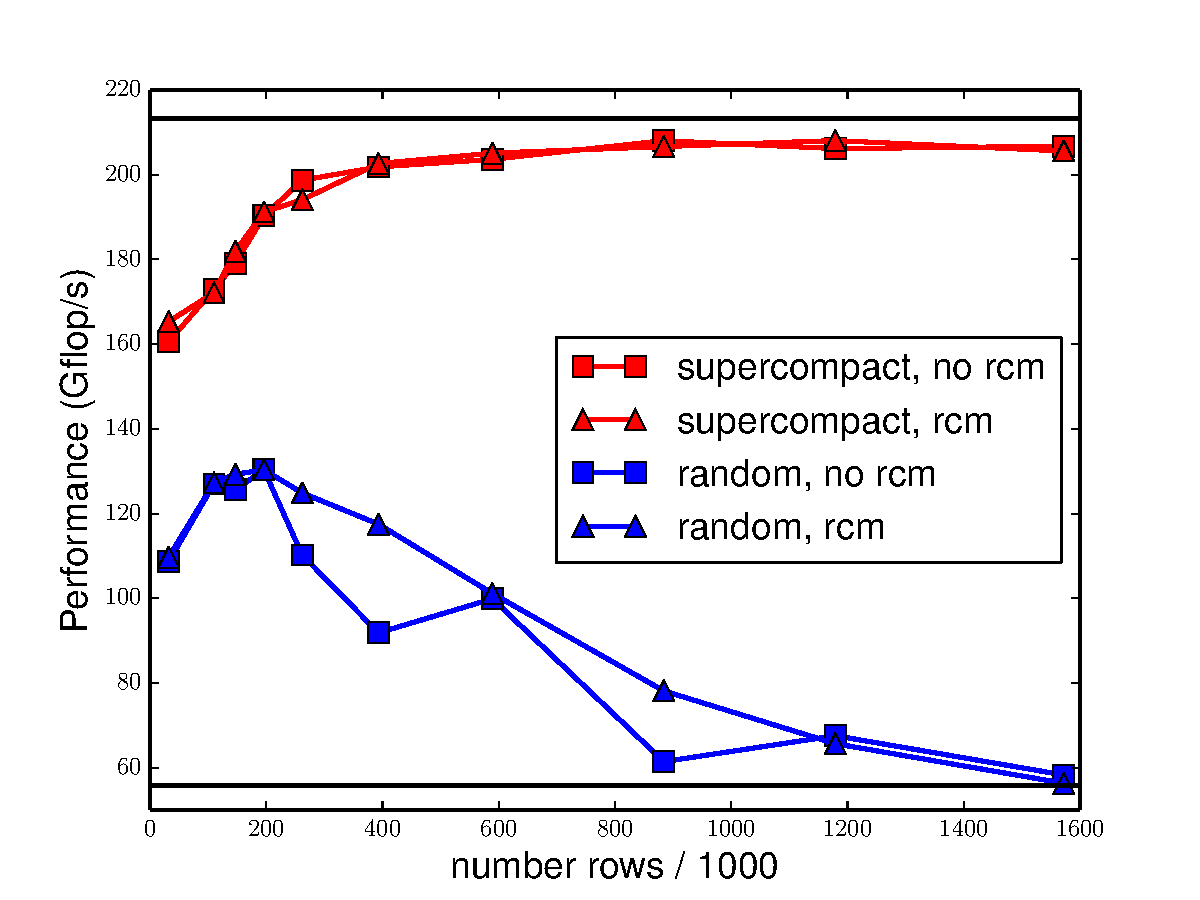
\includegraphics[width=.4\linewidth]{figures/random_supercompact.pdf}\label{fig:perf_ideal}}
% was width=.48
  \subfigure[Compact and RBFFD.]{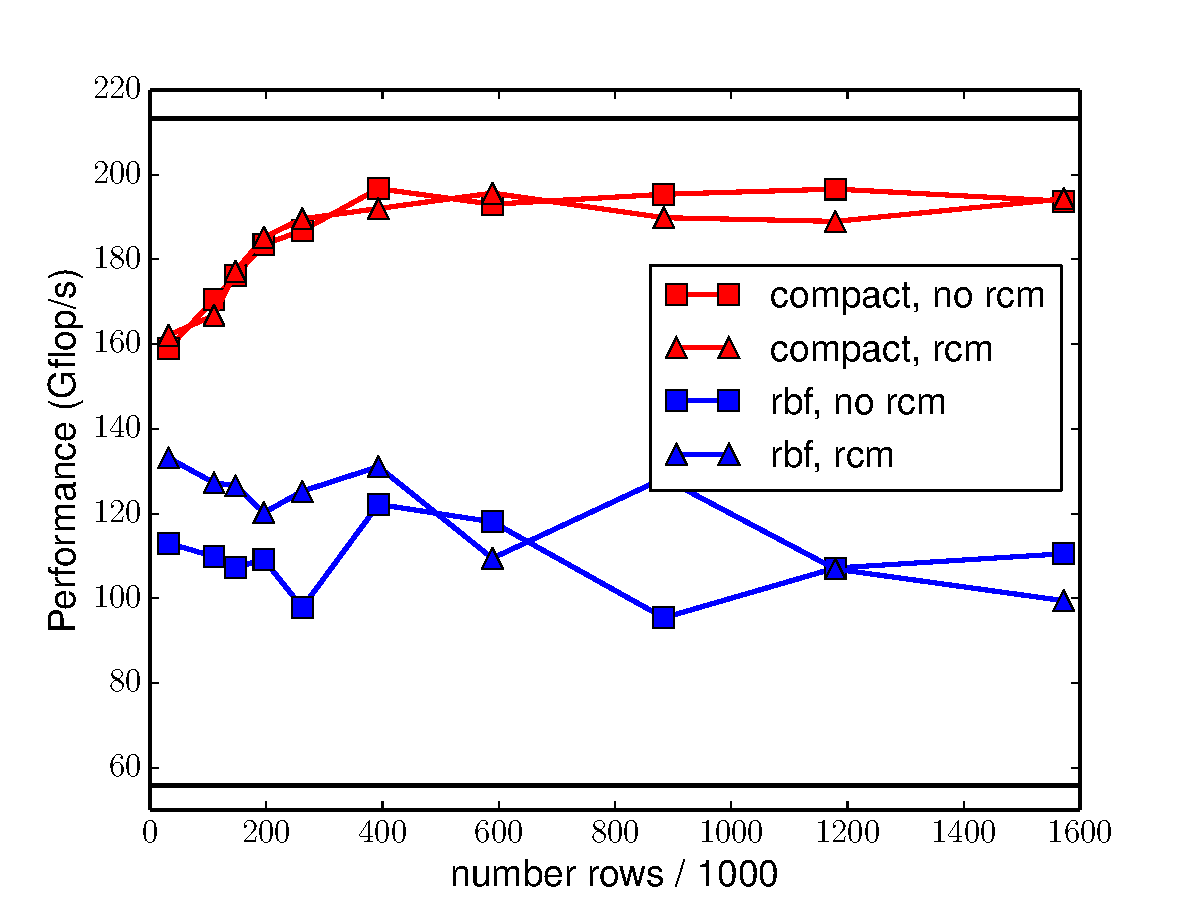
\includegraphics[width=.4\linewidth]{figures/rbf_compact.pdf}\label{fig:perf_realistic}}
  
  \caption{Performance of the manually vectorized code. The two
    horizontal lines depict the worst and the best predicted performances.}
  \label{fig:expe_types}
\end{figure*}



To summarize, using vector instructions appears necessary in order
to reach the highest bandwidth on the MIC architecture. For the instructions used
in a typical SpMV computation, one can expect a bandwidth between
140~GB/s to 160~GB/s. That is why we use in our estimations a best
achievable bandwidth of 150~GB/s despite the fact that a 
 code carefully crafted to maximize bandwidth can reach higher
values~\cite{Saule13-ARXIV}. 

\subsection{Instances}

The different matrices used to perform our experiments and analysis
are presented in Figure~\ref{fig:spy_plots}. The
\ttt{Supercompact} matrices (Figure~\ref{fig:supercompact}) have been
generated to only have nonzero elements in the first 32 columns of
the matrix. As a result, only 32 values of {\tt x} are read
from memory, and the expense associated with cache misses is removed from consideration. The cost associated with 
{\tt A} remains. The \ttt{Compact} matrices
(Figure~\ref{fig:compact}) are generated to have 32 nonzeros per row
centered around the diagonal and it represents the ideal case for many
applications that rely on sparse matrix vector multiplication. The nonzero
elements of the \ttt{Random}
matrices (Figure~\ref{fig:random}) see their nonzero elements
randomly (uniformly) distributed in the matrix; they represent the
worst case scenario for a cache-based architecture where the cache
reutilisation is the lowest from one row to the next.
The other type of matrix is used in derivative stencils in 3D
RBFFD calculations (Figure~\ref{fig:rbf3dnorcm} shows a $32$-point
stencil of a 3D $8^3$ grid).

We also apply a Reverse Cuthill-Mckee reordering to
all the matrices.  This ordering technique aims to reduce the
distance between the nonzeros and the diagonal, hopefully increasing 
the cache hit ratio.  The reordered version of the matrix can be
seen in Figure~\ref{fig:rbf3drcm}.

\vspace{-0.3em}
\subsection{Computations}

We now investigate the actual performance that we can obtain when
multiplying four vectors by four matrices in single
precision. Figure~\ref{fig:expe_types} presents results for different
types of matrices and also shows the minimum and maximum performance
predicted in Section~\ref{sec:model}. Figure~\ref{fig:perf_ideal}
gives the results for the {\tt supercompact} and {\tt random} matrices
that represent both the best and the worst case for such a practical 
computation. The {\tt supercompact} case peaks at
208~Gflop/s which is very close to the predicted peak
performance of 213~Gflop/s. Conversely the performance of the {\tt
  random} case decreases to 56~Gflop/s which is close to
the lowest predicted performance of 55~Gflop/s. One can see that RCM
ordering helps the {\tt random} case but the impact decreases when the
size of the matrix increases.

Figure~\ref{fig:perf_realistic} gives the results on the {\tt compact}
case, which represents the best realistic matrix one could find with very
structured grids and a
{\tt RBF} derivative matrix extracted from a real 3D application. In the {\tt
  compact} case, the performance can be as high as 195~Gflop/s, which is
within 15\% of the predicted  peak performance. The performance of the
{\tt RBF} case varies between 100 and 140~Gflop/s. Most of the
time, the RCM ordering provides an improvement which can be as high as
30~Gflop/s.

\begin{figure}[h]
% Figure 10
  \centering 
  
  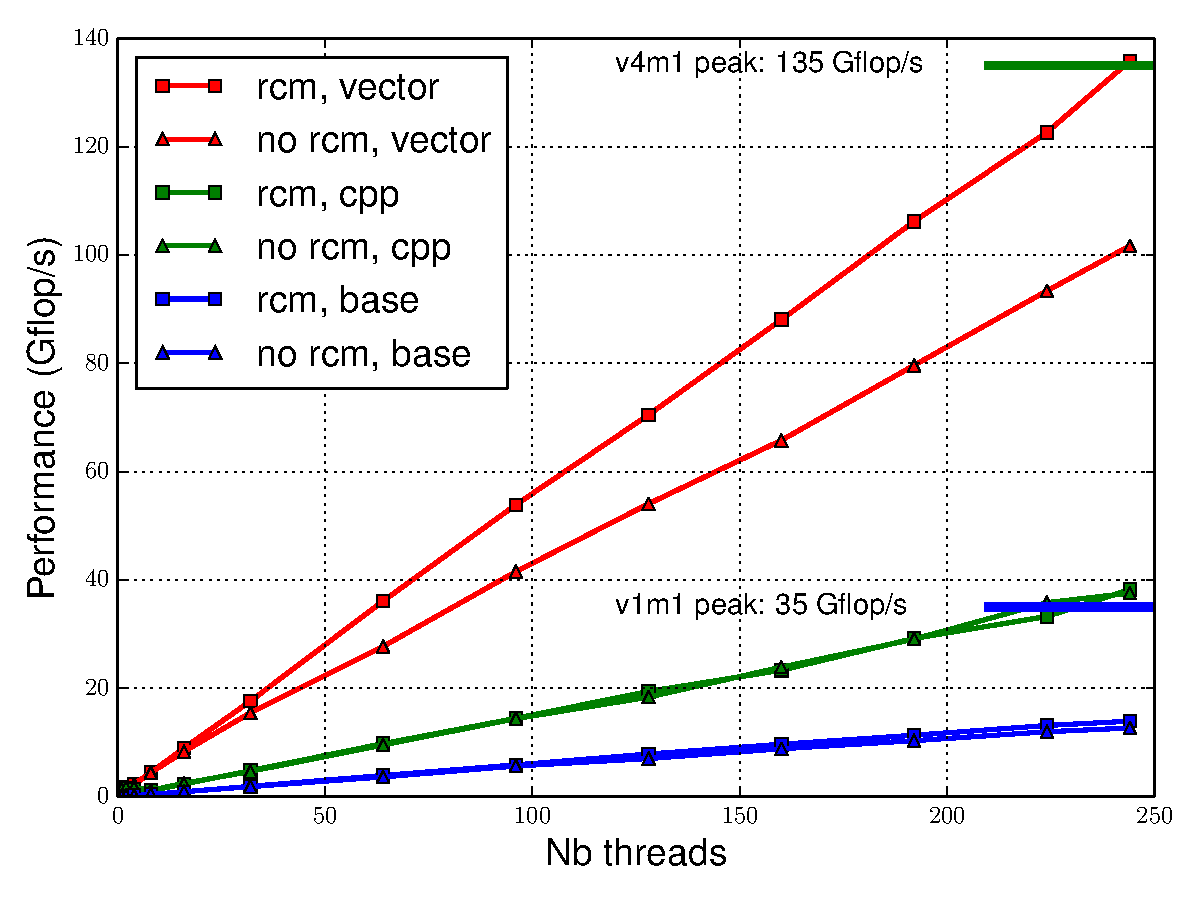
\includegraphics[width=.9\linewidth]{figures/mic_performance_nb_threads.pdf}

  \caption{Performance of $y=Ax$ for a RBF derivative stencil of a
    $96^3$ 3D grid. Classical "one-matrix one-vector" SpMV ($n_m=n_v=1$ given in blue) has low
    performance. The manually vectorized code (red) is 3.5 times
    faster than the compiler generated one (green). RCM ordering
    (squares) only improves the performance for our manually
    vectorized code.
    We also show peak theoretical performance for v1m1 and v4m1 on the MIC. 
    Not shown is the peak theoretical performance of 210 Gflops for v4m4. 
    }
  \label{fig:comparison_spmv}
  \label{fig:perf_mic}
\end{figure}

We finally investigate the central questions of this paper. Do we gain
actual performance by transforming classical SpMV computation into the
multiplication of four vectors by four matrices for the computation of the
derivative of RBFs? Does using manual vectorization improve actual
application performance? Figure~\ref{fig:comparison_spmv} compares the
performance achieved by a classical SpMV and by the multiplication of
four vectors by four matrices using either standard C++ code and our
optimized implementation. The
classical SpMV computation reaches 14~Gflop/s. 
The standard C++ implementation reaches a performance of 38~Gflop/s while our
optimized implementation almost reaches 140~Gflop/s. 
Notice that 
RCM ordering has no impact in the standard C++ implementation while it
provides a significant improvement in our manually vectorized
version. Thus, the C++ implementation is likely instruction-bound
while our manually vectorized implementation is most likely 
memory-bound. 

\ger{The main idea of this paper, computing 16 derivatives at a time,
can be applied on different architectures such as multiprocessor
multicore or GPU. To illustrate this fact, we conducted similar experiments
on Cascade at the Minnesota Supercomputing Institute
using two XEON E5 2670 nodes (8 cores, 2 threads and 20 Mbytes of L2
cache per core, with hyperthreading disabled.) The cores support the AVX instruction set. 
Both the compiler-generated code and the code written with the 
help of the AVX instruction set reach a read bandwidth of
85~GB/s. Using cache lines of 256 bits, we find a best/worst speeds of 4/20\; Gflops/s and 
50/120\; Gflops/s, respectively for the 1vec/1mat and 4vec/4mat cases. 
Our implementation on Cascade reaches 45 Gflops for the 4/4\, case, or 41\% of peak theoretical 
performance on this particular processor setup. For references, we achieve 
140/210=66\% of peak theoretical performance on the MIC. Note that peak performance 
is not that of the processor, but of the best possible algorithm on the processor. 
The gain in the 4/4 case with respect to 4x 1/1 case is respectively 4x on the MIC 
and 2.5x on the front end.  
}

\vspace{-0.5em}
\section{Conclusion}
\label{sec:ccl}

In the previous sections, we have explored the practical
implementation on an Intel Xeon Phi card of multiple derivative
operators acting on multiple vectors within the context of
RBFFD. Each derivative has an associated sparse matrix with a fixed
number of nonzeros on each row. While computing a single derivative of
multiple functions is rather common, we accelerate the algorithm further 
by considering multiple
matrices, with identical sparsity patterns, acting on multiple vectors. 
We specialize our study to four matrices and four derivatives,
with 16 outputs, computed as a sum of outer products.

Our implementation makes use of the IMCI MIC instruction set and
includes a number of swizzling and channel swapping operations, for an
extremely efficient tensor product implementation. 
\NOTE{From Evan: this is the first time $96^3$ is mentionned. Might wish to mention 
it earlier.} On a $96^3$ 3D
grid, it reaches a performance of 140~Gflop/s which is 2.7 times
faster than the best possible performance achievable for a single
vector and a single derivative and more than 7 times faster than a
practical implementation.

In future work, we will examine the effect of larger stencil sizes and
double precision. The presented performance does not reach the
predicted peak and we believe that common techniques from SpMV such as
cache partitioning can be successfully applied. We will also integrate
the techniques presented in this paper within a fluid simulation using
RBFFD. \ge{We will also look into developing a similar technique on the Kepler
family of GPUs, which offers swizzling and channeling operations.}

\section*{Acknowledgment}
Erlebacher acknowledges funding from NSF grant
DMS-\#0934331 (FSU), and the use of the MIC at FSU and at LCSE/U. Minnesota (provided by Prof. D. Yuen). NCAR is sponsored by NSF. 
Flyer acknowledges support of NSF grant DMS-0934317.


\bibliographystyle{plain} %{IEEEabrv,paper.bib}
\bibliography{paper, bollig}
\end{document}


